%
% 1-gruppe.tex -- Konzept einer Gruppe
%
% (c) 2022 Prof Dr Andreas Müller, OST Ostschweizer Fachhochschule
%
\section{Gruppen
\label{buch:gruppen:section:gruppe}}
\kopfrechts{Gruppe}
Die Translationsinvarianz des Definitionsbereiches $\mathbb{R}$
entsteht aus der Tatsache, dass die Addition einer Zahl
nicht aus $\mathbb{R}$ herausführt und sich auch umkehren lässt.
Sie basiert also darauf, dass es in $\mathbb{R}$ eine umkehrbare
Verknüpfung gibt.
Diese Idee wird von der algebraischen Struktur einer Gruppe eingefangen.

%
% 1-gruppe.tex -- Konzept einer Gruppe
%
% (c) 2022 Prof Dr Andreas Müller, OST Ostschweizer Fachhochschule
%

%
% Definition
%
\subsection{Definition
\label{buch:gruppen:subsection:definition}}
Der Begriff einer Gruppe soll alle Arten von invertierbaren Rechenoperationen
erfassen, also Addition/Subtraktion, Multiplikation/Division oder
die Matrixmultiplikation mit der inversen Matrix.
Die minimal nötigen Eigenschaften fasst die folgende Definition zusammen.

\begin{definition}
\label{buch:gruppen:definition:gruppe}
Eine {\em Gruppe} $G$ ist eine Menge mit einer Verknüpfung
$\cdot \colon G\times G\to G : (x,y) \mapsto xy $, welche folgende
Eigenschaften hat:
\begin{enumerate}
\item
Die Verknüpfung ist assoziativ, d.~h.~$(xy)z=x(yz)$ für alle
$x,y,z\in G$.
\item
Es gibt ein {\em neutrales Element} $e\in G$, für welches $ex=x$ für alle
$x\in G$ gilt.
\index{neutrales Element}%
\item 
Zu jedem $x\in G$ gibt es ein {\em inverses Element} $x^{-1}\in G$ mit der
Eigenschaft $x^{-1}x=e$.
\index{inverses Element}%
\end{enumerate}
\end{definition}

Man beachte, dass die Defiinition nicht verlangt, dass die Faktoren
vertauscht werden können. 

\begin{beispiel}
Die Menge $\operatorname{GL}_n(\mathbb{R})$ der invertierbaren
$n\times n$-Matrizien mit reellen Einträgen und der Matrixmultiplikation
heisst die {\em allgemeine lineare Gruppe}.
\index{allgemeine lineare Gruppe}%
\index{Gruppe!allgemeine lineare}%
Das neutrale Element von $\operatorname{GL}_n(\mathbb{R})$ ist die
Einheitsmatrix, das inverse Element einer Matrix
$A\in \operatorname{GL}_n(\mathbb{R})$
ist die inverse Matrix $A^{-1}$.
\end{beispiel}

%
% Abelsche Gruppen
%
\subsubsection{Abelsche Gruppen}
Die Definition einer Gruppe verlangt nicht, dass die Verknüpfung der
Gruppenelemente kommutativ sein müsste.
Tatsächlich haben die meisten Matrizengruppen, wie weiter unten als 
Beispiele besprochen werden, eine nicht kommutative Verknüpfung.
Es stellt sich aber heraus, dass Gruppen mit einer kommutativen
Verknüpfung zu einer besonders reichhaltigen harmonischen Analysis
führen.

\begin{definition}
\label{buch:gruppen:definition:abelsch}
Eine Gruppe $G$ heisst {\em abelsch}, wenn 
die Verknüpfung in der Gruppe kommutativ ist, wenn also
$xy=yx$ für alle $x,y\in G$ gilt.
\end{definition}

Die Verknüpfung einer abelschen Gruppe ist also {\em kommutativ}.
\index{kommutativ}%
Abelsche Gruppen werden oft additiv geschrieben, d.~h.~mit einem
Pluszeichen als $x+y$ für $x,y\in G$.
Das neutrale Element heisst dann auch das {\em Nullelement} und wird $0$
geschrieben: $x+0=x$ für alle $x\in G$.
Das inverse Element von $x$ heisst dann auch das
{\em entgegengesetzte Element} und wird $-x$ geschrieben. 
Es gilt $x+(-x)=0$ für alle $x\in G$.

\begin{beispiel}
Die Gruppe $(\mathbb{R},+)$ ist eine abelsche Gruppe.
Die Gruppe der von $0$ verschiedenen Zahlen mit der Multiplikation
$(\mathbb{R}^*,\cdot)$ ist eine abelsche Gruppe.
\end{beispiel}

\begin{beispiel}
Die {\em Gruppe der Drehwinkel} in der Ebene ist die Menge
\(
\mathbb{R}/2\pi\mathbb{Z}
=
(-\pi,\pi].
\)
Als Gruppenoperation dient die Addition von Winkeln, die Summe
$\alpha+\beta$ zweier Winkel $\alpha$ und $\beta$ muss dazu durch
Subtraktion oder Addition von Vielfachen von $2\pi$ ins Intervall
$(-\pi,\pi]$ zurückgebracht werden.
Neutrales Element ist $0$, das inverse Elemente ist $-\alpha$ mit
dem Spezialfall $-\pi=\pi$.
\end{beispiel}

\begin{beispiel}
Die von $0$ verschiedenen Element $\mathbb{C}^*$ mit der Multiplikation
ist eine Gruppe.
Das neutrale Element ist die Zahl $1\in\mathbb{C}^*$ und das inverse
Element zu $z\in\mathbb{C}^*$ ist $z^{-1}$.
\end{beispiel}

%
% Untergruppen
%
\subsubsection{Untergruppen}
Da man Drehungen auch mit Hilfe von komplexen Zahlen beschreiben kann,
kann man die Gruppe der Drehwinkel auch als Menge von komplexen Zahlen
schreiben, nämlich als die Menge
\[
S^1
=
\{z\in\mathbb{C}\mid |z|=1\}
\]
der komplexen Zahlen vom Betrag $1$.
Die Gruppenoperation in $S^1$ ist die gleiche wie die Operation
in $\mathbb{C}^*$, von der $S^1$ eine Teilmenge ist.

\begin{definition}
\label{buch:gruppen:definition:def:untergruppe}
Sei $G$ eine Gruppe und $H\subset G$ eine Teilmenge derart,
dass mit jedem $x,y\in H$ auch $xy$ und $x^{-1}$ in $H$ sind.
Dann heisst $H$ eine {\em Untergruppe} von $G$.
\index{Untergruppe}%
\end{definition}

Jede Gruppe enthält als kleinste Untergruppe immer die Gruppe $G$,
die {\em triviale Gruppe}, die nur aus dem neutralen Element
$\{e\}\subset G$ besteht.

%
% Homomorphismen
%
\subsubsection{Homomorphismen}
Die Exponentialabbildung
\[
\exp
\colon
\mathbb{R}/2\pi\mathbb{Z} \to S^1
:
\alpha \mapsto e^{i\alpha}
\]
bildet Drehwinkel auf komplexe Zahlen vom Betrag $1$ ab.
Die Gruppenoperation bleibt dabei erhalten, es gilt
\[
\exp(\alpha + \beta)
=
e^{i(\alpha+\beta)}
=
e^{i\alpha}
e^{i\beta}
=
\exp(\alpha)
\exp(\beta).
\]
Das neutrale Element $0\in\mathbb{R}/2\pi\mathbb{Z}$ wird auf
das neutrale Element $1\in S^1$ abgebildet und das inverse
Element von $\exp(\alpha)$ ist
$ \exp(\alpha)^{-1} = \exp(-\alpha) $.
Ausserdem ist die Abbildung bijektiv.
Die Exponentialabbildung zeigt also, dass es zwischen den beiden
Gruppen $\mathbb{R}/2\pi\mathbb{Z}$ und $S^1$ nicht wirklich einen
Unterschied gibt.

Die Gruppe der Drehwinkel kann man auch als eine Matrizengruppe
verstehen, wie im folgenden Beispiel gezeigt wird.

\begin{beispiel}
Die Menge
\[
\operatorname{SO}(2)
=
\biggl\{
\begin{pmatrix}
\cos\alpha & -\sin\alpha \\
\sin\alpha &  \cos\alpha
\end{pmatrix}
\;
\bigg|
\;
\alpha\in\mathbb{R}
\biggr\}
\]
ist eine Gruppe mit der Matrixmultiplikation als Gruppenoperation,
der Einheitsmatrix als neutralem Element und der inversen Matrix
als inversem Element.
\end{beispiel}

Die Abbildung
\[
\varphi
\colon
\mathbb{R}/2\pi\mathbb{Z}
\to
\operatorname{SO}(2)
:
\alpha
\mapsto
D_\alpha
=
\begin{pmatrix}
\cos\alpha & -\sin\alpha \\
\sin\alpha &  \cos\alpha
\end{pmatrix}
\]
transportiert die Gruppenoperation von $\mathbb{R}/2\pi\mathbb{Z}$
nach $\operatorname{SO}(2)$ denn es gilt
\[
\varphi(\alpha)\varphi(\beta)
=
\begin{pmatrix}
\cos\alpha & -\sin\alpha \\
\sin\alpha &  \cos\alpha
\end{pmatrix}
\begin{pmatrix}
\cos\beta & -\sin\beta \\
\sin\beta &  \cos\beta
\end{pmatrix}
=
\begin{pmatrix}
\cos(\alpha+\beta) & -\sin(\alpha+\beta) \\
\sin(\alpha+\beta) &  \cos(\alpha+\beta)
\end{pmatrix}
=
\varphi(\alpha+\beta).
\]
Auch ist $\varphi(0)$ die Einheitsmatrix und
$\varphi(-\alpha)=\varphi(\alpha)^{-1}$.

\begin{definition}
\label{buch:gruppen:definition:def:homomorphismus}
Eine Abbildung $\varphi\colon G\to H$ zwischen zwei Gruppen $G$ und $H$
heisst ein {\em Homomorphismus}, wenn
$\varphi(gh)=\varphi(g)\varphi(h)$ gilt für alle $g,h\in G$
\end{definition}

Die Bildmenge $\varphi(G)$ eines Homomorphismus ist automatisch eine
Untergruppe $\varphi(G)\subset H$.
Sind $\varphi(x)$ und $\varphi(y)$ Elemente in $\varphi(G)$,
dann ist auch $\varphi(x)\varphi(y)=\varphi(xy)\in\varphi(G)$.

%
% Der Kern eines Homomorphismus
%
\subsubsection{Der Kern eines Homomorphismus}
Ist $\varphi\colon G\to H$ ein Homomorphismus von Gruppen und
$U\subset H$ eine Untergruppe von $H$, dann bilden die Elemente
\[
\varphi^{-1}(U)
=
\{g\in G\mid \varphi(g)\in U\}
\]
eine Untergruppe.
Sind nämlich $g_1,g_2\in\varphi^{-1}(U)$, dann ist
\[
\varphi(g_1g_2)
=
\varphi(g_1)\varphi(g_2)
\in U,
\]
da $U$ eine Untergruppe ist.
Dann ist aber auch $g_1g_2\in\varphi^{-1}(U)$, was zeigt, dass
$\varphi^{-1}(U)$ eine Untergruppe von $G$ ist.
Sie heisst die {\em Urbildgruppe} von $U$ unter dem Homomorphismus
$\varphi$.

Besonders wichtig ist die Urbildgruppe der trivialen Gruppe.

\begin{definition}
\label{buch:gruppen:definition:def:kern}
Der Kern eines Homomorphismus $\varphi \colon G\to H$ ist die
Untergruppe
\[
\ker \varphi = \varphi^{-1}(\{e\}).
\]
\end{definition}

Der Kern eines Homomorphismus kann dazu verwendet werden zu beurteilen,
ob der Homomorphismus injektiv ist.
Wenn nämlich $\varphi(x)=\varphi(y)$ ist, dann ist auch
\[
e
=
\varphi(x)\varphi(y)^{-1}
=
\varphi(xy^{-1})
\quad\Rightarrow\quad
xy^{-1} \in\ker\varphi.
\]
Es folgt also genau dann $x=y$, wenn der Kern $\ker\varphi$ nur
das neutrale Element enthält.


%
% 12-endlich.tex -- Konzept einer Gruppe
%
% (c) 2022 Prof Dr Andreas Müller, OST Ostschweizer Fachhochschule
%

%
% Endliche Gruppen
%
\subsection{Endliche Gruppen
\label{buch:gruppen:subsection:endliche-gruppen}}
Für theoretische Überlegungen sind die kontinuierliche
Fourier-Transformation auf Gruppen wie $\mathbb{R}$ oder
$\mathbb{R}/2\pi\mathbb{Z}$ besonders Leistungsfähig, weil hier die
ganze Macht der Analysis zur Konstruktion der orthonormierten Basis
zur Verfüfung steht.
In Ingenieuranwendungen reduziert man die unendlichdimensionalen
Vektorräume dagegen gerne auf endliche Menge, so dass man mit
Vektoren und Matrizen rechnen kann.
Dafür müssen endliche Gruppen als Definitionsbereiche für die Funktionen
gefunden werden.

%
% Die zyklischen Gruppen \mathbb{Z}/n\mathbb{Z}
%
\subsubsection{Die zyklischen Gruppen $\mathbb{Z}/n\mathbb{Z}$}
Für die diskrete Fourier-Analysis besonders wichtig sind die zyklischen
Gruppen.

\begin{definition}
\label{buch:gruppen:endliche-gruppen:def:zyklisch}
Die Gruppe
\[
\mathbb{Z}/n\mathbb{Z}
=
\{0,1,2,\dots,n-1\}
\]
der Reste modulo $n$ mit der Addition von Resten ist eine abelsche
Gruppe.
\end{definition}

Die zyklischen Gruppen können auch als multiplikativ geschriebene
Untergruppen der von $0$ verschiedenen komplexen Zahlen geschrieben
werden.
Dazu verwendet man die Exponentialfunktion:
\[
C_n
=
\{ e^{2\pi ik/n}\mid k=0,1,\dots,n-1\}.
\]
Die Exponentialabbildung
\[
\exp
\colon
\mathbb{Z}/n\mathbb{Z}
\to
C_n
:
k\mapsto e^{2\pi ik/n}
\]
ist ein Homomorphismus, denn
\[
\exp(k+l)
=
e^{2\pi i(k+l)/n}
=
e^{2\pi ik/n}
e^{2\pi il/n}
=
\exp(k)\exp(l).
\]
Die Reste werden auf verschiedene Ecken eines regelmässigen
$n$-Ecks in der komplexen Ebene abgebildet, die Abbildung $\exp$
ist daher auch eine Bijektion.
Die additiv geschriebene Gruppe $\mathbb{Z}/n\mathbb{Z}$ und
die multiplikativ geschriebene Gruppe $C_n$ sind also isomorph.

%
% Die zyklischen Gruppen als Kern
%
\subsubsection{Die zyklischen Gruppen als Kern}
Die Gruppe $C_n$ wurde früher schon als Bild der Gruppe
$\mathbb{R}/2\pi\mathbb{Z}$ unter der Exponentialabbildung 
in $\mathbb{C}^*$ erkannt worden.
Man kann sie aber auch als Kern eines geeignet gewählten Homomorphismus
verstehen.

Die Abbildung
\[
\varphi
\colon
S^1\to S^1
:
z\mapsto z^n
\]
ist ein Homomorphismus, denn es ist ja $\varphi(z_1z_2)=(z_1z_2)^n
= z_1^nz_2^n=\varphi(z_1)\varphi(z_2)$.
Der Kern von $\varphi$ besteht aus den komplexen Zahlen mit der 
Eigenschaft $z^k=1$, das sind genau die Elemente von $C_n$.

%
% Permutationsgruppen
%
\subsubsection{Permutationsgruppen}
Die Menge $[n]=\{1,2,\dots,n\}$ hat $n$ Elemente.
Wir betrachten die Menge aller invertierbaren Abbildungen
$\varphi\colon [n] \to [n]$.
Zwei solche Abbildungen $\varphi$ und $\psi$ können zusammengesetzt
werden, oder sie können invertiert werden $\varphi^{-1}$.
Tatsächlich ist die Menge 
\[
S_n = \{\varphi\colon [n] \to [n]\mid \text{$\varphi$ ist invertierbar} \}
\]
eine Gruppe, sie heisst die {\em Permutationsgruppe von $n$ Elementen}
oder die {\em symmetrische Gruppe}.

Permutationen können besonders effizient als Matrizen mit zwei Zeilen
geschrieben werden.
Eine Abbildung $\varphi\colon [n]\to[n]$ bildet $i\in [n]$ auf $\varphi(u)$
ab, was man als die Matrix
\[
\varphi
=
\begin{pmatrix}
1&2&3&\dots&n\\
\varphi(1)&\varphi(2)&\varphi(3)&\dots&\varphi(n)
\end{pmatrix}
\]
schreiben kann.
Um die Komposition von zwei Abbildungen $\varphi$ und $\psi$ zu bestimmen,
kann man die beiden Matrizen übereinander schreiben und die Spalten der
unteren Matrix so sortieren, dass sie mit den Elementen in der unteren
Zeile der oberen übereinstimmen:
\[
\begin{aligned}
\varphi
&=
\begin{pmatrix}1&2&3&4\\2&3&1&4\end{pmatrix}
\\
\psi
&=
\begin{pmatrix}1&2&3&4\\3&2&4&1\end{pmatrix}
\end{aligned}
\quad\Rightarrow\quad
\psi\circ \varphi
=
\left\{
\begin{array}{c}
\displaystyle\begin{pmatrix}1&2&3&4\\2&3&1&4\end{pmatrix}\\
\displaystyle\begin{pmatrix}1&2&3&4\\3&2&4&1\end{pmatrix}
\end{array}
\right\}
=
\left\{
\begin{array}{c}
\displaystyle\begin{pmatrix}1&2&3&4\\2&3&1&4\end{pmatrix}\\
\displaystyle\begin{pmatrix}2&3&1&4\\2&4&3&1\end{pmatrix}
\end{array}
\right\}
=
\begin{pmatrix}
1&2&3&4\\
2&4&3&1
\end{pmatrix}.
\]

Die inverse Abbildung findet man, indem man die beiden Zeilen vertauscht
und die Spalten so sortiert, dass die Elemente in der ersten Zeile
wieder aufsteigend sind.
Zum Beispiel
\[
\varphi
=
\begin{pmatrix}
1&2&3&4&5\\
1&3&5&2&4
\end{pmatrix}
\quad\Rightarrow\quad
\varphi^{-1}
=
\begin{pmatrix}
1&3&5&2&4\\
1&2&3&4&5
\end{pmatrix}
=
\begin{pmatrix}
1&2&3&4&5\\
1&4&2&5&3
\end{pmatrix}.
\]
Die Zusammensetzung von $\varphi$ und $\varphi^{-1}$ ist
\[
\varphi\circ\varphi^{-1}
=
\left\{
\begin{array}{c}
\displaystyle
\begin{pmatrix}
1&2&3&4&5\\
1&4&2&5&3
\end{pmatrix}
\\
\displaystyle
\begin{pmatrix}
1&2&3&4&5\\
1&3&5&2&4
\end{pmatrix}
\end{array}
\right\}
=
\left\{
\begin{array}{c}
\displaystyle
\begin{pmatrix}
1&2&3&4&5\\
1&4&2&5&3
\end{pmatrix}
\\
\displaystyle
\begin{pmatrix}
1&4&2&5&3\\
1&2&3&4&5
\end{pmatrix}
\end{array}
\right\}
=
\begin{pmatrix}
1&2&3&4&5\\
1&2&3&4&5
\end{pmatrix}
=
e.
\]

\begin{definition}
Eine {\em Transposition} $\tau\in S_n$ ist eine Permutation, die genau
zwei Elemente vertauscht und alle anderen Elemente fest bleiben.
\end{definition}

Die Permutationsgruppe $S_n$ ist für $n>2$ nicht abelsch, denn die beiden
Transpositionen
\[
\tau_{12}
=
\begin{pmatrix}
1&2&3&\dots&n\\
2&1&3&\dots&n
\end{pmatrix}
,
\qquad
\tau_{23}
=
\begin{pmatrix}
1&2&3&\dots&n\\
1&3&2&\dots&n
\end{pmatrix}
\]
haben die Produkte
\begin{align*}
\tau_{12}
\circ
\tau_{23}
&=
\begin{pmatrix}
1&2&3&\dots&n\\
2&3&1&\dots&n
\end{pmatrix}
&&\text{und}&
\tau_{23}
\circ
\tau_{12}
&=
\begin{pmatrix}
1&2&3&\dots&n\\
3&1&2&\dots&n
\end{pmatrix},
\end{align*}
die verschieden sind.

Die Permutationsgruppen können als die ``ultimativen'' endlichen Gruppen
im folgenden Sinne betrachtet werden.
Sei $G=\{e=g_1,g_2,\dots,g_n\}$ irgend eine endliche Gruppe, und $g\in G$
ein Gruppenelement.
Für jedes Element $g_i$ ist $gg_i=g_{\pi(i)}$ wieder ein Gruppenelement.
Damit wird eine Permutation $\pi\in S_n$ definiert.
Die Gruppe $G$ kann damit als eine in $S_n$ Gruppe von Permutationen
betrachtet werden.
Jede endliche Gruppe ist somit eine Untergruppe von $S_n$.
Für die Zwecke der harmonischen Analysis ist diese Betrachtungsweise
allerdings nicht besonders ergibig.

%
% Permutationsmatrizen
%
\subsubsection{Permutationsmatrizen}
Die Permutationsgruppe hat auch eine wichtige Rolle bei der Definition
der Determinante mit Hilfe des Entwicklungssatzes, wie zum Beispiel
in \cite[Kapitel~4]{buch:linalg} ausgeführt wird.
Darin spielen die Transpositionen eine besondere Rolle, da die
Vertauschungen zweier Spalten einer Matrix das Vorzeichen ihrer
Determinanten umkehrt.
Tatsächlich können die Permutationen von $S_n$ auch als
$n\times n$-Matrizen geschrieben werden.
Der Permutation $\pi\in S_n$ wird die lineare Abbildung
$\mathbb{R}^n\to\mathbb{R}^n$ zugeordnet, die den Standardbasisvektor
$e_k$ auf den Standardbasisvektor $e_{\sigma(k)}$ abbildet.
Die zugehörige Matrix $P_\sigma$ hat die Matrixelemente
\[
(P_\sigma)_{ik} 
=
\begin{cases}
1&\qquad i = \pi(k)\\
0&\qquad\text{sonst}.
\end{cases}
\]
Die Verknüpfung von Permutationen wird zur Matrixmultiplikation,
die Abbildung $\sigma \mapsto P_\sigma$ ist ein Homomorphismus
von der Gruppe $S_n$ in die Gruppe der Permutationsmatrizen.
Man sagt auch, die Permutationen werden durch Matrizen dargestellt oder
die Abbildung, die einer Permutation $\sigma$ die zugehörige
Permutationsmatrix $P_\sigma$ zuordnet, ist eine Darstellung der
Gruppe $S_n$ im Vektorraum $\mathbb{R}^n$.

Die Spalten einer Permutationsmatrix sind die permutierten
Standardbasisvektoren.
Man kann die Permutation rückgängig machen, indem man die Spalten
paarweise geeignet vertauscht.
Die Determinante der Matrix ändert dabei jedesmal das Vorzeichen.
Am Ende des Prozesses steht die Einheitsmatrix mit Determinante $1$.
Insbesondere ist die Determinanten einer Permutationsmatrix $\pm 1$.

\begin{definition}
\index{Vorzeichen einer Permutation}%
\index{Signum einer Permutation}%
Das {\em Vorzeichen} oder {\em Signum} einer Permutation
$\operatorname{sgn}(\sigma)$
ist die Determinante der zugehörigen Permutationsmatrix:
$\operatorname{sgn}(\sigma)=\det P_\sigma$.
Eine Permutation heisst {\em gerade}, wenn $\operatorname{sgn}(\sigma)=1$ ist,
sei heisst {\em ungerade}, wenn $\operatorname{sgn}(\sigma)=-1$ ist.
\index{gerade Permutation}%
\index{ungerade Permutation}%
\end{definition}

Die Permutationsmatrix $P_\tau$ einer Transposition $\tau$ hat nur
zwei vertauschte Spalten, also ist $\operatorname{sgn}(\tau)=\det P_\tau=-1$.
Der oben beschrieben Prozess, mit dem erkannt wurde, dass die Determinante
einer Permutationsmatrix $\pm 1$ sein muss, zeigt noch mehr.

\begin{satz}
Jede Permutation $\sigma$ kann als Produkt von Transpositionen
geschrieben werden.
Das Signum einer Permutation ist genau dann $+1$, wenn $\sigma$
als Zusammensetzung einer geraden Anzahl von Transpositionen
geschrieben werden kann.
Es ist $-1$, wenn $\sigma$ Zusammensetzung einer ungeraden Anzahl
von Transpositionen geschrieben werden kann.
\end{satz}

%
% Die alternierende truppe
%
\subsubsection{Die alternierende Gruppe}
Das Vorzeichen $\operatorname{sgn}$ ist die Zusammensetzung zweier
Homomorphismen, nämlich der Abbildung $\sigma\to P_\sigma$
und der Determinante.
Die Produktregel für Determinanten besagt, dass $\det(AB)=\det(A)\det(B)$,
die Determinante macht also aus der Matrixmultiplikation das Produkt von
reellen Zahlen.
Für zwei Permutationen $\sigma,\varrho\in S_n$ gilt daher für die Signa
\[
\operatorname{sgn}(\sigma\varrho)
=
\det P_{\sigma\varrho}
=
\det(P_\sigma P_\varrho)
=
\det(P_\sigma)\det( P_\varrho)
=
\operatorname{sgn}(\sigma)
\operatorname{sgn}(\varrho).
\]
Die Zusammensetzung von Homomorphismen ist auch wieder ein Homomorphismus.

Die Menge
\[
A_n
=
\{ \sigma\in S_n \mid \operatorname{sgn}(\sigma) = 1 \}
=
\ker
\operatorname{sgn}
\]
ist als Kern eines Homomorphismus $S_n\to\mathbb{R}$
eine Untergruppe von $S_n$, denn für $\sigma_1,\sigma_2\in S_n$ ist auch
\(
\operatorname{sgn}(\sigma_1\sigma_2)
=
\operatorname{sgn}(\sigma_1)
\operatorname{sgn}(\sigma_2)
=
1\cdot 1
\),
und daher auch $\sigma_1\sigma_2\in S_n$.
Ausserdem ist 
\(
\operatorname{sgn}(\sigma^{-1})=\det P_{\sigma^{-1}}
=
\det P_\sigma^{-1}
=
(\det P_\sigma)^{-1}
=
1^{-1}=1,
\)
somit ist mit $\sigma\in A_n$ auch $\sigma^{-1}\in A_n$.
Die Menge $A_n$ heisst die {\em alternierende Gruppe}.


%
% 13-lie.tex -- Lie-Gruppen
%
% (c) 2022 Prof Dr Andreas Müller, OST Ostschweizer Fachhochschule
%

%
% Lie-Gruppen
%
\subsection{Lie-Gruppen
\label{buch:gruppen:subsection:lie-gruppen}}
Die endlichen Gruppen unterscheiden sich grundlegend von der Gruppe
der Drehwinkel.
In $\mathbb{R}$, $\mathbb{R}/2\pi\mathbb{Z}$, $S^1$ und $\mathbb{C}^*$
steht nicht nur die aus der Gruppenoperation abgeleitete algebraische
Struktur zur Verfügung.

%
% Topologische Gruppen
%
\subsubsection{Topologische Gruppen}
Vielmehr kann man auch von konvergenten Folgen von Gruppenelementen
sprechen und davon, ob eine Abbildung zwischen diesen Gruppen
stetig ist.
Man nennt eine solche Gruppe eine {\em topologische Gruppe}.
\index{topologische Gruppe}%

\begin{beispiel}
Die Menge
\(
\mathbb{Q}^*
=
\mathbb{Q} \setminus\{0\}
\)
ist eine Gruppe mit der Multiplikation als Gruppenoperation.
\end{beispiel}

Die Gruppe $\mathbb{Q}^*$ ist eine topologische Gruppe.
Als Teilmenge von $\mathbb{Q}$ ist klar, was eine Cauchy-Folge in
$\mathbb{Q}^*$ ist.
Es gibt aber auch Cauchy-Folgen in $\mathbb{Q}^*$, die nicht konvergieren.
Die Folge
\[
x_0=1,\;
x_{n+1} = \frac12\biggl(x_n+\frac{2}{x_n}\biggr),\; n\in\mathbb{N},
\]
ist eine Folge von rationalen Zahlen, die gegen einen Fixpunkt der
Funktion
\[
x\mapsto f(x)=\frac12\biggl(x+\frac{2}{x}\biggr)
\]
konvergiert.
Durch Multiplikation mit $x$ findet man
\[
x=f(x)
\quad\Rightarrow\quad
x^2=\frac12 x^2 + 1
\quad\Rightarrow\quad
\frac12x^2=1
\quad\Rightarrow\quad
x^2=2
\quad\Rightarrow\quad
x=\!\sqrt{2},
\]
insbesondere ist der Grenzwert nicht in $\mathbb{Q}^*$.

\begin{definition}
\label{buch:gruppen:gruppe:def:topgruppe}
Eine topologische Gruppe $G$ ist eine Gruppe $G$, deren Verknüpfungsabbildung
$(x,y)\mapsto xy$ und das inverse Element $x\mapsto x^{-1}$ stetig sind.
Für konvergente Folgen $x_n\to x$ und $y_n\to y$ in $G$ gilt dann
\begin{align*}
\lim_{n\to \infty} x_ny_n &= \lim_{n\to\infty} x_n \lim_{n\to\infty} y_n = xy
\\
\lim_{n\to \infty} x_n^{-1} &= (\lim_{n\to\infty} x_n)^{-1} = x^{-1}
\end{align*}
\end{definition}

%
% Koordinatensysteme
%
\subsubsection{Koordinatensysteme}
Für Funktionen auf der Gruppe $\mathbb{R}$ ist sogar die Ableitung
definiert.
Eine solche lässt sich auch für Funktionen auf den Gruppen 
$S^1$ und $\operatorname{SO}(2)$ definieren, indem man diese Gruppen
mit einer geeigneten Parametrisierung beschreibt.
Die der Ableitungsbegriff nur für Funktionen $\mathbb{R}^n \to\mathbb{R}^m$
definiert ist, können solche Parametrisierungen dazu dienen,
die Gruppe mit einem Koordinatensystem auszustatten und anschliessend
die Ableitungen auf der Basis dieser Koordinaten zu definieren.

Die Bestrebung, einer Gruppe mit Hilfe von Koordinaten eine differenzierbare
Struktur zu verpassen, ist natürlich viel allgemeiner, auch
gewöhnliche im dreidimensionalen Raum eingebetteten Flächen
benötigen ein Koordinatensystem, damit man Ableitungen von Kurven
auf der Fläche unabhängig von der Einbettung der Fläche in den
dreidimensionalen Raum studieren kann.
Ziel dieses Abschnitts ist daher, beliebigen Mengen ein Koordinatensystem
zu geben.

Ein $n$-dimensionales Koordinatensystem einer Menge $U$ besteht
aus Funktionen $x_i\colon U\mathbb{R}$ für $i=1,\dots,n$, die für
jeden Punkt $p\in U$ die Koordinaten $x_i(p),i=1,\dots,n,$ berechnen.
Fasst man diese Funktionen $x_i$ zusammen in ein $n$-Tupel, ergibt
sich eine Abbildung $x\colon U\mathbb{R}^n:p\mapsto (x_1(p),\dots,x_n(p))$.
Damit Punkte mit Hilfe ihrer Koordinaten unterscheidbar sind, muss
die Abbildung injektiv sein: wenn die Punkte $p$ und $q$ verschieden sind,
dann unterscheiden sich auch $x_i(p)$ und $x_i(q)$ für mindestens ein $i$
und die $n$-Tupel $x(p)$ und $x(q)$ unterscheiden sich in mindestens
einer Koordinate.

\begin{beispiel}
Die Menge $U=\mathbb{R}^+\times \mathbb{R}^+$ der Paare von positiven
Zahlen ist eine offene Teilmenge von $\mathbb{R}^2$, man kann also die
Zahlen $u,v$ selbst als Koordinaten verwenden.
Neben diesem offensichtlichen Koordinatensystem gibt es aber mindestens
noch zwei weitere einfache Koordinatensysteme, die die Menge
gleichermassen beschreiben.

Die Abbildung
\[
y
\colon
U \to \mathbb{R}^n
:
(u,v) \mapsto (\log u,\log v)
\]
ist injektiv. 
Diese Karte hat noch eine weitere besondere Eigenschaft.
Die Menge $U$ erhält eine Gruppenstruktur mit der Verknüpfung
\begin{align*}
(u_1,v_1)\cdot (u_2,v_2)&=(u_1u_2,v_1v_2)
\intertext{mit dem neutralen Element $(1,1)$ und dem inversen}
(u,v)^{-1}&= (u^{-1},v^{-1})
\qquad\Rightarrow\qquad
(u,v)^{-1}(u,v) = (u^{-1},v^{-1})(u,v) = (u^{-1}u,v^{-1}v) = (1,1).
\end{align*}
Die Abbildung $y$ ist dann sogar ein Homomorphismus von der Gruppe $U$ 
in die additive Gruppe $\mathbb{R}^2$.

Ein weiteres Koordinatensystem ist die Abbildung
\[
z
\colon
U\to\mathbb{R}^2
:
(u,v)\mapsto \biggl(uv, \frac{u}{v}\biggr).
\]
Die koordinaten sind ebenfalls positiv und die Abbildung wird durch
\[
(z_1,z_2) \mapsto (\!\sqrt{z_1z_2},\!\sqrt{z_1/z_2})
\]
invertiert.
Auch dieses Koordinatensystem ist ein Homomorphismus der multiplikativen
Gruppe $U$ in die Gruppe $U$, denn
\begin{align*}
z(p_1p_2)
&=
z\bigl(
(u_1,v_1)
(u_2,v_2)
\bigr)
=
z\bigl(
(u_1u_2,v_1v_2)
\bigr)
\\
&=
\biggl( u_1u_2v_1v_2 , \frac{u_1u_2}{v_1v_2}\biggr)
=
\biggl( u_1v_1\cdot u_2v_2, \frac{u_1}{v_1}\cdot\frac{u_2}{v_2}\biggr)
=
\biggl( u_1v_1,\frac{u_1}{v_1} \biggr)
\biggl( u_2v_2,\frac{u_2}{v_2} \biggr)
\\
&=
z(p_1)
z(p_2).
\qedhere
\end{align*}
\end{beispiel}

Das Beispiel zeigt, dass es viele verschiedene Koordinatensysteme
auf einer Menge geben kann, die sogar mit der Gruppenstruktur verträglich
sein können.
Betrachtet man aber Mengen die die Kugeloberfläche, dann wird schnell
klar, dass es oft kein Koordinatensystem für die ganze Menge gibt.
Kugelkoordinaten zum Beispiel verwenden die geographische Länge und 
Breite, aber die Pole haben keine wohldefinierte geogrphische Länge.
Im Allgemeinen können Koordinatensysteme also nur lokal für eine offene
Teilmenge der ganzen Menge konstruiert werden.
Kartographen tun genau dies für die Erdoberfläche: Sie konstruieren
ein Koordinatensystem für eine kleine Teilmenge der Erdoberfläche.

\begin{definition}
\label{buch:gruppen:gruppe:def:karte}
Eine $n$-dimensionale {\em Karte} $\alpha$ für eine offene Menge
$U_\alpha\subset M$ ist eine injektive Abbildung
$\varphi_\alpha\colon U\to \mathbb{R}^n$.
\end{definition}

\begin{beispiel}
Für die Menge $\mathbb{R}^n$ ist die Abbildung
$U=\mathbb{R}^n\to \mathbb{R}^n$, die dem $x\in\mathbb{R}^n$ auf
$x$ abbildet eine geeignete Karte, die auf ganz $\mathbb{R}^n$ ein
Koordinatensystem definiert.
\end{beispiel}

\begin{beispiel}
\label{buch:gruppen:gruppe:bsp:kugel}
\begin{figure}
\centering
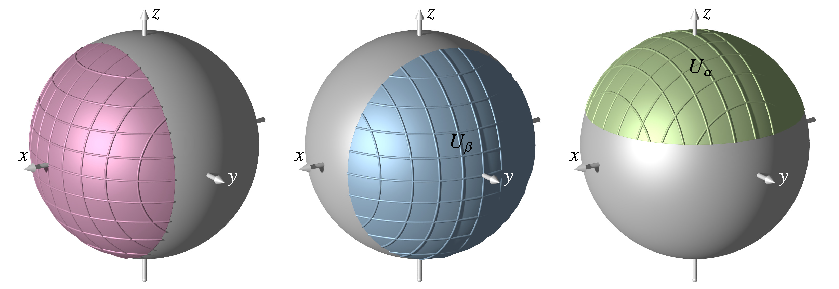
\includegraphics{chapters/030-gruppen/images/kugelkarten.pdf}
\caption{Drei verschiedene Karten auf einer Kugeloberfläche jeweils in
einer Umgebung der Schnittpunkte der Kugeloberfläche mit einer
Achse.
\label{buch:gruppen:gruppe:fig:kugelkarten}}
\end{figure}
Die Menge $S^2 = \{(x,y,z)\mid x^2+y^2+z^2=1\}$ ist eine Kugeloberfläche.
In der Umgebung $U_\alpha = \{(x,y,z)\in S^2\mid x^2+y^2<0.9\wedge z>0\}$
des Nordpoles ist die Abbildung
\[
\varphi_\alpha
\colon
U_\alpha
:
(x,y,z)\mapsto (x,y)
\]
eine gute Karte, sie deckt aber alle anderen Pole überhaupt nicht ab.
In der Umgebung $U_\beta = \{(x,y,z)\in S^2\mid x^2+z^2<0.9\wedge y>0\}$
des Punktes $(0,1,0)$ ist die Abbildung
\[
\varphi_\beta
\colon
U_\beta
:
(x,y,z)\mapsto (x,z)
\]
dagegen eine gute Karte.
So kann für jeden Pol eine Karte gefunden werden, die in 
Abbildung~\ref{buch:gruppen:gruppe:def:karte} dargestellt sind.
\end{beispiel}

Das Beispiel zeigt, dass die vollständige Beschreibung einer Menge
eine Vielzahl von Karten benötigen kann.
Aus den Koordinatenfunktionen werden dann andere Eigenschaften der
Menge abgeleietet.
Dies kann jedoch nur funktionieren, wenn im Überschneidungsbereich
zweier Koordinatensysteme, die gleichen Eigenschaften abgeleitet
werden können.
Im nächsten Abschnitt wird genau dieses Problem für die
Charakterisierung der Differenzierbarkeit von Funktionen auf der
Menge adressiert.

%
% Ableitungen
%
\subsubsection{Ableitungen}
\begin{figure}
\centering
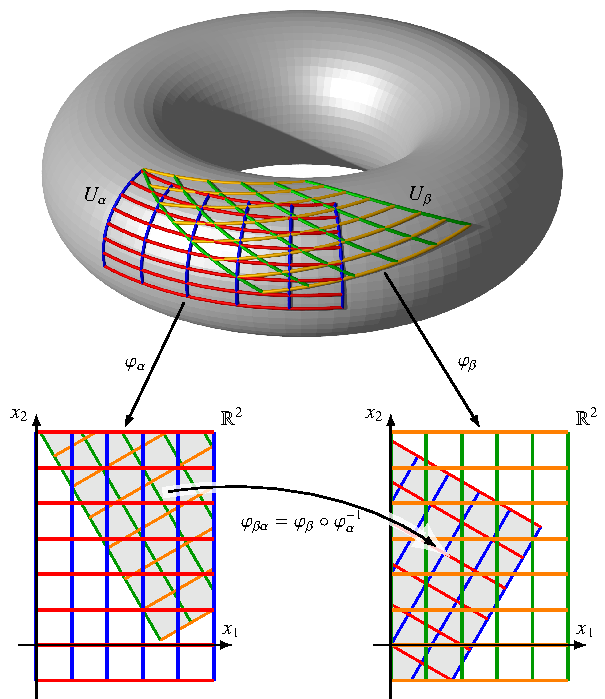
\includegraphics{chapters/030-gruppen/images/karten.pdf}
\caption{Kartenwechsel für zwei Karten auf einem Torus
\label{buch:gruppen:gruppe:fig:kartenwechsel}}
\end{figure}
Die Karten sollen der Menge $M$ ein Koordinatensystem geben, mit dem
man Ableitungen von Funktionen definieren kann.
Dazu ist notwendig, dass verschiedene Karten auf die gleiche
Ableitung führen.
Seien $x_i$ und $y_i$ Koordinaten für eine offene Teilmenge von $M$,
und $f$ eine Funktionen auf $M$.
In dieser Menge können die Koordinaten $x_i$ als Funktionen der 
Koordinaten $y_k$ in der Form $x_i(y_1,\dots,y_k)$ schreiben.
Ebenso kann man $f$ durch die Koordinaten $x_i$ ausdrücken, dies
schreiben wir als $f(x_1,\dots,x_n)$, oder durch die Koordinaten $y_i$,
dies schreiben wir als $f(y_1,\dots,y_n)$.
Die Ableitung der Funktion $f$ nach den Koordinaten $y_i$ muss nach
der Kettenregel
\begin{equation}
\frac{\partial f}{\partial y_i}
=
\sum_{k=1}^n
\frac{\partial f}{\partial x_k} \frac{\partial x_k}{\partial y_i}
\label{buch:gruppen:gruppe:eqn:kettenregel}
\end{equation}
auch durch die Ableitungen von $f$ nach den Koordinaten $y_i$
ausgedrückt werden können.
Die Formel~\ref{buch:gruppen:gruppe:eqn:kettenregel} ist aber nur sinnvoll,
wenn die Ableitungen $\partial x_k/\partial y_i$ alle existieren.
Die Kartenwelchselabbildung $y\mapsto x$ muss also differenzierbar sein.
Die Koordinatenumrechnung zwischen zwei Karten müssen also differenzierbare
Abbildungen sein.

Seien also
$\varphi_\alpha\colon U_\alpha \to \mathbb{R}^n$
und
$\varphi_\beta\colon U_\beta \to \mathbb{R}^n$
zwei Karten, deren Definitionsbereiche $U_\alpha$ und $U_\beta$ sich
schneiden.
Sie statten also beide die Menge $U_{\alpha\beta}=U_\alpha\cap U_\beta$
mit einem Koordinatensystem aus.
Die Koordinatenwechselabbildung
\[
\varphi_{\beta\alpha}
=
\varphi_\beta
\circ
\varphi_\alpha^{-1}
\colon
\varphi_\alpha(U_\alpha\cap U_\beta)
\to
\varphi_\beta(U_\alpha\cap U_\beta)
\]
ist eine Abbildung zwischen offenen Teilmengen von $\mathbb{R}^n$.
Man sagt, der Kartenwechsel ist differenzierbar, wenn $\varphi_{\beta\alpha}$
differenzierbar ist.
Der Kartenwechsel in der umgekehrten Richtung ist $\varphi_{\alpha\beta}$.

\begin{definition}
\label{buch:gruppen:gruppe:def:atlas}
Ein {\em differenzierbarer Atlas} von $M$ ist eine Menge von Karten derart,
dass alle Kartenwechselabbildungen differenzierbar sind.
\end{definition}

\begin{definition}
\label{buch:gruppen:gruppe:def:diffman}
Eine {\em differenzierbare Mannigfaltigkeit} ist eine Menge $M$ mit einem
differenzierbaren Atlas derart, dass jeder Punkt von $M$ im
Definitionsgebiet mindestens einer Karte liegt.
\end{definition}

Eine differenzierbare Mannigfaltigkeit ist also eine Menge, die in
einer Umgebung jedes Punktes mit mindestens einem Koordinatensystem
ausgestattet werden kann auf eine Art, dass die Umrechnung zwischen
verschiedenen Koordinatensystemen immer differenzierbar ist.

\begin{beispiel}
Die reelle Achse $\mathbb{R}$ ist eine differenzierbare Mannigfaltigkeit,
sie lässt sich mit einer einzigen Karte parametrisieren.
\end{beispiel}

\begin{beispiel}
Die Kreislinie $S^1$ in der komplexen Ebene ist eine differenzierbare
Mannigfaltigkeit, Karten können wie folgt konstruiert werden.
Die Abbildung $\mathbb{R}\to S^1: x\mapsto e^{ix}$ bildet die ganze
reelle Achse auf die Kreislinie ab.
Die Abbildung ist allerdings nicht umkehrbar, weil $x$-Werte, die sich
um Vielfache von $2\pi$ unterscheiden, auf den gleichen Punkt in $S^1$
abgebildet werden.
Zu jedem Punkt $x\in\mathbb{R}$ gibt es aber ein Intervall
$U_x=(x-1,x+1)$, welches bijektiv auf eine Teilmenge von $S^1$
abgebildet wird.
Die Exponentialabbildung von $U_x\to S^1$ wie auch die Umkehrabbildung
von der Bildmenge zurück in $U_x$ sind stetig.
Die Koordinaten, die verschiedene solche Karten einem Punkt der Kreislinie
zuordnen können, unterscheiden sich immer um Vielfache von $2\pi$.
Die Koordinatenwechsel-Abbildung zwischen zwei Karten $U_x$ und $U_y$
sind also Abbildungen der Form $x\mapsto x+2\pi k$ mit $k\in\mathbb{Z}$,
also sicher differenzierbar.
Damit ist ein differenzierbarer Atlas für $S^1$ konstruiert, $S^1$
ist eine differenzierbare Mannigfaltigkeit.
\end{beispiel}

\begin{beispiel}
\begin{figure}
\centering
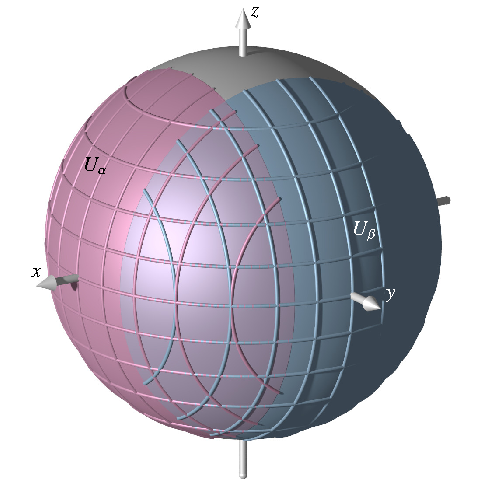
\includegraphics{chapters/030-gruppen/images/kugelschnitt.pdf}
\caption{Zwei Karten der Kugeloberfläche und deren Schnittbereich.
Differenzierbarkeit von Funktionen auf der Kugeloberfläche kann mit
Hilfe der Karten nur dann definiert werden, wenn die Kartenwechselabbildung
$\varphi_\alpha\circ\varphi_\beta^{-1}$ und
$\varphi_\beta\circ\varphi_\alpha^{-1}$ differenzierbare Abbildungen
zwischen offenen Mengen in $\mathbb{R}^n$ sind.
\label{buch:gruppen:gruppe:fig:kugelkartenwechsel}}
\end{figure}
Die Ableitung von Funktionen auf einer Kugeloberfläche muss auf 
die Beschreibung der Funktion in einer Karte mit Hilfe der dortigen
Koordinaten zurückführen.
Dazu ist notwendig, dass die Kartenwelchselabbildungen differenzierbar
sind.
Für die in Beispiel~\ref{buch:gruppen:gruppe:bsp:kugel} gezeigten
Karten auf der Kugeloberfläche ist dies leicht nachzurechnen.
Das in Abbildung~\ref{buch:gruppen:gruppe:fig:kugelkartenwechsel}
hat die Kartenwechselfunktion
\[
\varphi_\beta
\circ
\varphi_\alpha^{-1}
\colon
\varphi_\alpha(U_\alpha\cap U_\beta)
\to
\varphi_\beta(U_\alpha\cap U_\beta)
:
(x,z) \mapsto (x,\!\sqrt{1-x^2-z^2}),
\]
die offensichtlich differenzierbar ist, solange $x^2+z^2<1$ ist.
\end{beispiel}

%
% Differenzierbare Abbildungen
%
\subsubsection{Differenzierbare Abbildungen}
Ein differenzierbarer Atlas erlaubt jetzt auch Abbildungen zwischen
verschiedenen Mannigfaltigkeiten zu definieren.
Sind $M$ und $N$ differenzierbare Mannigfaltigkeiten der Dimension $m$
bzw.~$n$ und $f\colon M\to N$ eine Abbildung.
Ist $x\in M$ ein Punkt in $M$, dann gibt es eine Karte
$\varphi_\alpha\colon U_\alpha\to\mathbb{R}^m$ mit $x\in U_\alpha$
und eine Karten $\psi_\gamma\colon V_\gamma\to\mathbb{R}^n$ mit
$f(x)\in V_\gamma$.
In einer Umgebung von $\varphi_\alpha(x)$ kann die Abbildung $f$
in den Koordinaten als
\[
f_{\gamma,\alpha}
=
\psi_\gamma\circ f \circ \varphi_\alpha^{-1}
\]
geschrieben werden.
Als Abbildung einer offenen Menge in $\mathbb{R}^m$ in eine offene
Menge in $\mathbb{R}^n$ ist wohldefiniert, was es heisst, dass die
Abbildung differenzierbar ist.

Wählt man andere Karten $\varphi_\beta\colon U_\beta\to\mathbb{R}^n$
und $\psi_\delta\colon V_\delta\to\mathbb{R}^n$, die ebenfalls
das Urbild $x\in U_\beta$ und das Bild $f(x)\in V_\delta$ enthalten,
dann lässt sich die Funktion auch durch die neuen Koordinaten
\[
f_{\delta,\beta}
=
\psi_\delta\colon \circ f \circ\varphi_\beta^{-1}
\]
ausdrücken.
Natürlich muss auch $f_{\delta,\beta}$ differenuzierbar sein.
Diese beiden Arten, die Ableitung zu definieren, sind miteinander
konsistent, weil für die Zusammensetzung
\[
f_{\gamma,\alpha}
=
\psi_\gamma\circ\psi_\delta^{-1}
\circ
f_{\delta,\beta}
\circ
\varphi_\beta\circ\varphi_\alpha^{-1}
=
\psi_{\gamma\delta}
\circ
f_{\delta,\beta}
\circ
\varphi_{\beta\alpha}
\]
die Kettenregel gilt und die Kartenwechselabbildungen $\varphi_{\beta\alpha}$
und $\psi_{\gamma\delta}$ differenzierbar sind.

%
% Lie-Gruppen
%
\subsubsection{Lie-Gruppen}
Die Gruppen $S^1$ war als differenzierbare Mannigfaltigkeit erkannt
worden.
Damit die Struktur der Gruppe und die differenzierbare Struktur sinnvoll
miteinander verwendet werden können ist notwendig, dass die
Verknüpfungsabbildung $(x,y)\mapsto xy$ und die Umkehrabbildung
$x\mapsto x^{-1}$ nicht nur stetig, sondern sogar differenzierbar sind.

\begin{definition}
\label{buch:gruppen:gruppe:def:liegruppe}
Eine Lie-Gruppe ist eine Gruppe, die gleichzeitig eine differenzierbare
Mannigfaltigkeit ist derart, dass die Gruppenoperation
$G\times G\to G:(x,y)\mapsto xy$
und die Invertierung $G\to G: x\mapsto x^{-1}$ differenzierbare Abbildungen
sind.
\end{definition}

In den für die Gruppe $S^1$ konstruierten Karten ist die Verknüpfung die
Addition von Koordinaten und die Invertierung ist der Vorzeichenwechsel.
Beide sind differenzierbar, daher ist $S^1$ eine Lie-Gruppe.

%
% Koordinatensysteme auf Matrizengruppen
%
\subsubsection{Koordinatensysteme auf Matrizengruppen}
Die allgemeine lineare Gruppe $\operatorname{GL}_n(\mathbb{R})$
ist eine offene Teilmenge von $\mathbb{R}^{n\times n}$ ist.
Die Matrixelemente $a_{ik}$ sind daher auf natürliche Weise ein
Koordinatensystem auf der Gruppe $\operatorname{GL}_n(\mathbb{R})$.
Die Gruppenoperationen lassen sich als Summen von Produkten von
Matrixelementen schreiben.
Mit den Matrixelementen als Koordinaten folgt unmittelbar, dass
die Gruppenoperationen differenzierbare Abbildungen sind.

Alle anderen Matrizengruppen sind Teilmengen von
$\operatorname{GL}_n(\mathbb{R})$ niedrigerer Dimension.
Zum Beispiel besteht die Gruppe $\operatorname{SL}_n(\mathbb{R})$
aus den Matrizen mit Determinante $1$, der $(n^2-1)$-dimensionalen
Teilmenge von $\operatorname{GL}_n(\mathbb{R})$ bestehend aus
den Nullstellen der Gleichung $\det(A)-1=0$.
Die Gruppe $\operatorname{SO}(n)$ besteht aus den Matrizen, die
zusätzlich $A^tA=I$ erfüllen.
Da $A^tA$ eine symmetrische Matrix ist, sind dies
$n(n+1)/2$ unabhängige Bedinungen.
Da daraus auch $\det A=\pm$ folgt, ist die $n(n-1)/2$ Dimension der Gruppe
$\operatorname{SO}(n)$, denn
\[
n^2 - \frac{n(n+1)}2
=
\frac{2n^2-n^2-n}{2}
=
\frac{n^2-n}2
=
\frac{n(n-1)}2.
\]
Da diese Einschränkungen ausserdem differenzierbar sind und in der
Einheitsmatrix keine Singularitäten haben, kann man davon ausgehen,
dass diese Teilmengen Untermannigfaltigkeiten sind.

Kann man auf kanonische Art Karten für die Matrizengruppen
konstruieren?
Die Matrixform der Rodrigues-Formel (\cite[p.~438]{buch:linalg})
beschreibt Drehungen des dreidimensionalen Raumes um die Achse mit
Richtung des Einheitsvektors $\vec{u}$ und um den Drehwinkel $\alpha$a
durch die Matrix
\[
D_{\vec{u},\alpha}
=
\begin{pmatrix}
 1-(1-c)(1-u_1^2) & -su_3+(1-c)u_1u_2 &  su_2+(1-c)u_1u_3 \\
 su_3+(1-c)u_1u_2 &  1-(1-c)(1-u_2^2) & -su_1+(1-c)u_2u_3 \\
-su_2+(1-c)u_1u_3 &  su_1+(1-c)u_2u_3 &  1-(1-c)(1-u_3^2) 
\end{pmatrix}
\]
beschrieben werden kann.
Der Vektor $\vec{u}$ ist ein Einheitsvektor und daher $\vec{u}\in S^2$
ein Punkt auf einer Kugel.
Wählt man auf der Kugel eine Karte, kann man daraus zusammen mit den
Drehwinkeln eine Karte für die Drehmatrizen konstruieren.
Dies zeigt, dass $\operatorname{SO}(3)$ eine differenzierbare
Mannigfaltigkeit ist.

Die Konstruktion des vorangeangenen Absatzes ist nicht direkt
auf andere Matrizengruppen verallgemeinerbar.
Man kann aber zeigen, dass in einer Umgebung der Einheitsmatrix
sich die Matrizen einer Matrizengruppe mit Hilfe der Exponentialreihe
schreiben lassen (siehe auch \cite[Abschnitt~9.4.4]{buch:linalg}).
Zum Beispiel sind die Matrizen $A\in \operatorname{SL}_n(\mathbb{R})$
in einer Umgebung von $I$ von der Form
\(
e^U
\),
wobei
die  Matrix $U$ Spur $\operatorname{tr}{U}=0$ haben muss.
Die Menge der Matrizen mit Spur $0$ ist eine $(n^2-1)$-dimensionale
Teilmenge von $M_{n}(\mathbb{R})$.
Die Umkehrabbildung der Exponentialabbildung kann daher als Karte
in einer Umgebung von $I$ dienen.

Ganz allgemein ist die Exponentialabbildung immer eine lokal
invertierbare Abbildung von der Lie-Algebra einer Matrizengruppe
in die Lie-Gruppe.
Da die Lie-Algebra ein $\mathbb{R}$-Vektorraum ist, kann eine
lokale Umkehrabbildung um die Einheitsmatrix $I$ als Karte mit
Werten in der Lie-Algebra dienen.
Für die Gruppe $\operatorname{SO}(3)$ zum Beispiel besteht die
Lie-Algebra aus antisymmetrischen Matrizen, also Matrizen
der Form
\[
U
=
\begin{pmatrix}
  0  & -u_3 &  u_2 \\
 u_3 &   0  & -u_1 \\
-u_2 &  u_1 &   0
\end{pmatrix}.
\]
Die Exponentialabbildung ordnet der Matrix $U$ die Matrix $e^U$
zu, die nach der Exponentialform der Rodrigues-Formel 
(\cite[p.~483]{buch:linalg}) die Drehmatrix der Drehung um die
Achse mit Richtung $\vec{u}^0$ und mit Drehwinkel $\alpha=|\vec{u}|$
ist, wobei $\vec{u}$ der Vektor mit den Komponenten $u_1$, $u_2$ und
$u_3$ ist.
Das Tripel $(u_1,u_2,u_3)$ bildet also ein gutes Koordinatensystem
für eine Umgebung der Einheitsmatrix in der Gruppe $\operatorname{SO}(3)$.

Die aus der Lie-Algebra konstruierten Karten zeigen noch mehr.
Da die Exponentialabbildung beliebig oft differenzierbar ist und die
Matrixmultiplikation durch Polynome höchstens zweiten Grades in
den Matrixelementen ausgedrückt werden kann, sind die Koordinatenwechsel
immer beliebig oft differenzierbar.
Die Matrizengruppen sind also sogar beliebig oft differenzierbare
Mannigfaltiketen. 
Es ist daher zulässig, sich für die Zwecke der nachfolgenden Diskussionen
immer auf beliebig oft differenzierbare Funktionen einzuschränken.
Andere, weniger oft differenzierbare Funktionen können durch
solche Funktionen beliebig genau approximiert werden.


%
% 1r-funktionenaufg.tex -- Funktionen auf G
%
% (c) 2022 Prof Dr Andreas Müller, OST Ostschweizer Fachhochschule
%

%
% Funktionen auf einer Gruppe
%
\subsection{Funktionen auf einer Gruppe
\label{buch:gruppen:subsection:funktionen}}
In diesem Abschnitt ist $G$ eine Gruppe, die wir multiplikativ
schreiben.
Die harmonische Analysis handelt von der Analyse von Funktionen.
Im Falle einer Lie-Gruppe kann man zusätzlich sinnvoll von Ableitungen
der Funktionen sprechen.
Wir definieren daher

\begin{definition}
\label{buch:gruppen:gruppe:def:funktionenaufgruppe}
Die Menge der stetigen reell- und komplexwertigen Funktionen wird mit
$C_{\mathbb{R}}(G)$ bzw.~$C_{\mathbb{C}}(G)$ bezeichnet.
Ist $G$ eine Lie-Gruppe, dann ist
$C_{\mathbb{R}}^\infty(G)$ die Menge der unendlich oft differenzierbaren
reellwertigen Funktionen auf $G$,
$C_{\mathbb{C}}^\infty(G)$ ist die Menge der unendlich oft differenzierbaren
komplexwertigen Funktionen.
\end{definition}

Die Gruppenstruktur ermöglich, lineare Operatoren auf $C_{\mathbb{R}}(G)$
und $C_{\mathbb{C}}(G)$ zu definieren.

\begin{definition}
\label{buch:gruppen:gruppe:def:translation}
Für $s\in G$ ist $T_s$ die Abbildung
\[
T_s
\colon
C_{\mathbb{R}}(G) \to C_{\mathbb{R}}(G)
:
f \mapsto T_sf
\quad
\text{mit}
\quad
(T_sf)(x) = f(s^{-1}x).
\]
Sie heisst die {\em Translation} um $s\in G$.
\end{definition}

Die Translation ist natürlich linear, denn
\begin{align*}
(T_s(f+g))(x)
&=
(f+g)(s^{-1}x)
\\
&=
f(s^{-1}x) + g(s^{-1}x)
=
(T_sf)(x) + (T_sg)(x)
&&\Rightarrow&
T_s(f+g)&=T_sf+T_sg
\\
(T_s(\lambda f))(x)
&=
\lambda f(s^{-1}x)
=
\lambda (T_sf)(x)
&&\Rightarrow&
T_s\lambda f
&=
\lambda T_sf
\end{align*}

%
% Eigenvektoren von T_s
%
\subsubsection{Eigenfunktionen des Translationsoperators}
Tatsächlich wurden in früheren Kapiteln Funktionen verwendet, die
bezüglich der Translation besondere Eigenschaften hatten.
Zum Beispiel sind die Funktionen $f(x)=e_k(x)=e^{ikx}$ auf $G=\mathbb{R}$
Eigenfunktionen des Translationsoperators, denn
\[
(T_se_k)(x)
=
e^{ik(x-s)}
=
e^{iks}e^{ikx}
=
e^{-iks} e_k(x).
\]
Insbesondere ist $e_k$ eine Eigenfunktion von $T_s$ mit Eigenwert
$\lambda=e^{-iks}$, also $T_se_k = \lambda e_k$.

%
% Gruppenstruktur der Translationen
%
\subsubsection{Gruppenstruktur der Translationen}
Wir berechnen die Zusammensetzung zweier Translationen ist $T_s$ und $T_t$.
Um $T_sT_t$ zu berechnen, muss zunächst die Funktion $T_tf$ bestimmt werden.
Es ist $(T_tf)(x) = f(t^{-1}x)$.
Die Translation $T_sg$ einer beliebigen Funktion auf dem Element $y\in G$
ist $(T_sg)(y)=g(s^{-1}y)$.
Setzt man $g=T_tf$ ein, ergibt sich
\[
(T_sT_tf)(x)
=
(T_tf)(s^{-1}x)
=
f(t^{-1}s^{-1}x)
=
f((st)^{-1}x)
=
(T_{st}f)(x),
\]
also $T_sT_t=T_{st}$.

%
% Rechtsoperation der Gruppe auf 
%
\subsubsection{Rechtsoperation von $G$ auf $C(G)$}
Die Operation $T_s$ ist genauer die Links-Translation, die Gruppenoperation
wirkt auf das Argument von links.
Für eine abelsche Gruppe spielt die Reihenfolge der Operanden keine
Rolle, für eine nichtabelsche Gruppe ergibt sich jedoch ein Unterschied.

\begin{definition}
Der Operator $R_s\colon C(G)\to C(G)$ der Rechts-Translation ist definiert
durch
\[
R_s
\colon
C_{\mathbb{R}}(G)\to C_{\mathbb{R}}(G)
:
f \mapsto R_sf
\quad\text{mit}\quad
(R_sf)(x) = f(xs).
\]
\end{definition}

Die Zusammensetzung von $R_s$ und $R_t$ kann ganz ähnlich wie für
$T_s$ und $T_t$ berechnet werden.
Zunächst ist $R_sg(y) = g(ys)$.
Wendet man dies auf $g=R_tf$ mit $g(x)=(R_tf)(x)=f(xt)$ an, bekommt man
\[
(R_sR_tf)(x)
=
(R_sg)(x)
=
g(xs)
=
(R_tf)(xs)
=
f(xst)
=
(R_{st}f)(x)
\]
oder kurz $R_sR_t=R_{st}$.






%%
%% Definition
%%
%\subsection{Definition
%\label{buch:gruppen:subsection:definition}}
%Der Begriff einer Gruppe soll alle Arten von invertierbaren Rechenoperationen
%erfassen, also Addition/Subtraktion, Multiplikation/Division oder
%die Matrixmultiplikation mit der inversen Matrix.
%Die minimal nötigen Eigenschaften fasst die folgende Definition zusammen.
%
%\begin{definition}
%\label{buch:gruppen:definition:gruppe}
%Eine {\em Gruppe} $G$ ist eine Menge mit einer Verknüpfung
%$\cdot \colon G\times G\to G : (x,y) \mapsto xy $, welche folgende
%Eigenschaften hat:
%\begin{enumerate}
%\item
%Die Verknüpfung ist assoziativ, d.~h.~$(xy)z=x(yz)$ für alle
%$x,y,z\in G$.
%\item
%Es gibt ein {\em neutrales Element} $e\in G$, für welches $ex=x$ für alle
%$x\in G$ gilt.
%\index{neutrales Element}%
%\item 
%Zu jedem $x\in G$ gibt es ein {\em inverses Element} $x^{-1}\in G$ mit der
%Eigenschaft $x^{-1}x=e$.
%\index{inverses Element}%
%\end{enumerate}
%\end{definition}
%
%Man beachte, dass die Defiinition nicht verlangt, dass die Faktoren
%vertauscht werden können. 
%
%\begin{beispiel}
%Die Menge $\operatorname{GL}_n(\mathbb{R})$ der invertierbaren
%$n\times n$-Matrizien mit reellen Einträgen und der Matrixmultiplikation
%heisst die {\em allgemeine lineare Gruppe}.
%\index{allgemeine lineare Gruppe}%
%\index{Gruppe!allgemeine lineare}%
%Das neutrale Element von $\operatorname{GL}_n(\mathbb{R})$ ist die
%Einheitsmatrix, das inverse Element einer Matrix
%$A\in \operatorname{GL}_n(\mathbb{R})$
%ist die inverse Matrix $A^{-1}$.
%\end{beispiel}
%
%%
%% Abelsche Gruppen
%%
%\subsubsection{Abelsche Gruppen}
%Die Definition einer Gruppe verlangt nicht, dass die Verknüpfung der
%Gruppenelemente kommutativ sein müsste.
%Tatsächlich haben die meisten Matrizengruppen, wie weiter unten als 
%Beispiele besprochen werden, eine nicht kommutative Verknüpfung.
%Es stellt sich aber heraus, dass Gruppen mit einer kommutativen
%Verknüpfung zu einer besonders reichhaltigen harmonischen Analysis
%führen.
%
%\begin{definition}
%\label{buch:gruppen:definition:abelsch}
%Eine Gruppe $G$ heisst {\em abelsch}, wenn 
%die Verknüpfung in der Gruppe kommutativ ist, wenn also
%$xy=yx$ für alle $x,y\in G$ gilt.
%\end{definition}
%
%Die Verknüpfung einer abelschen Gruppe ist also {\em kommutativ}.
%\index{kommutativ}%
%Abelsche Gruppen werden oft additiv geschrieben, d.~h.~mit einem
%Pluszeichen als $x+y$ für $x,y\in G$.
%Das neutrale Element heisst dann auch das {\em Nullelement} und wird $0$
%geschrieben: $x+0=x$ für alle $x\in G$.
%Das inverse Element von $x$ heisst dann auch das
%{\em entgegengesetzte Element} und wird $-x$ geschrieben. 
%Es gilt $x+(-x)=0$ für alle $x\in G$.
%
%\begin{beispiel}
%Die Gruppe $(\mathbb{R},+)$ ist eine abelsche Gruppe.
%Die Gruppe der von $0$ verschiedenen Zahlen mit der Multiplikation
%$(\mathbb{R}^*,\cdot)$ ist eine abelsche Gruppe.
%\end{beispiel}
%
%\begin{beispiel}
%Die {\em Gruppe der Drehwinkel} in der Ebene ist die Menge
%\(
%\mathbb{R}/2\pi\mathbb{Z}
%=
%(-\pi,\pi].
%\)
%Als Gruppenoperation dient die Addition von Winkeln, die Summe
%$\alpha+\beta$ zweier Winkel $\alpha$ und $\beta$ muss dazu durch
%Subtraktion oder Addition von Vielfachen von $2\pi$ ins Intervall
%$(-\pi,\pi]$ zurückgebracht werden.
%Neutrales Element ist $0$, das inverse Elemente ist $-\alpha$ mit
%dem Spezialfall $-\pi=\pi$.
%\end{beispiel}
%
%\begin{beispiel}
%Die von $0$ verschiedenen Element $\mathbb{C}^*$ mit der Multiplikation
%ist eine Gruppe.
%Das neutrale Element ist die Zahl $1\in\mathbb{C}^*$ und das inverse
%Element zu $z\in\mathbb{C}^*$ ist $z^{-1}$.
%\end{beispiel}
%
%%
%% Untergruppen
%%
%\subsubsection{Untergruppen}
%Da man Drehungen auch mit Hilfe von komplexen Zahlen beschreiben kann,
%kann man die Gruppe der Drehwinkel auch als Menge von komplexen Zahlen
%schreiben, nämlich als die Menge
%\[
%S^1
%=
%\{z\in\mathbb{C}\mid |z|=1\}
%\]
%der komplexen Zahlen vom Betrag $1$.
%Die Gruppenoperation in $S^1$ ist die gleiche wie die Operation
%in $\mathbb{C}^*$, von der $S^1$ eine Teilmenge ist.
%
%\begin{definition}
%\label{buch:gruppen:definition:def:untergruppe}
%Sei $G$ eine Gruppe und $H\subset G$ eine Teilmenge derart,
%dass mit jedem $x,y\in H$ auch $xy$ und $x^{-1}$ in $H$ sind.
%Dann heisst $H$ eine {\em Untergruppe} von $G$.
%\index{Untergruppe}%
%\end{definition}
%
%Jede Gruppe enthält als kleinste Untergruppe immer die Gruppe $G$,
%die {\em triviale Gruppe}, die nur aus dem neutralen Element
%$\{e\}\subset G$ besteht.
%
%%
%% Homomorphismen
%%
%\subsubsection{Homomorphismen}
%Die Exponentialabbildung
%\[
%\exp
%\colon
%\mathbb{R}/2\pi\mathbb{Z} \to S^1
%:
%\alpha \mapsto e^{i\alpha}
%\]
%bildet Drehwinkel auf komplexe Zahlen vom Betrag $1$ ab.
%Die Gruppenoperation bleibt dabei erhalten, es gilt
%\[
%\exp(\alpha + \beta)
%=
%e^{i(\alpha+\beta)}
%=
%e^{i\alpha}
%e^{i\beta}
%=
%\exp(\alpha)
%\exp(\beta).
%\]
%Das neutrale Element $0\in\mathbb{R}/2\pi\mathbb{Z}$ wird auf
%das neutrale Element $1\in S^1$ abgebildet und das inverse
%Element von $\exp(\alpha)$ ist
%$ \exp(\alpha)^{-1} = \exp(-\alpha) $.
%Ausserdem ist die Abbildung bijektiv.
%Die Exponentialabbildung zeigt also, dass es zwischen den beiden
%Gruppen $\mathbb{R}/2\pi\mathbb{Z}$ und $S^1$ nicht wirklich einen
%Unterschied gibt.
%
%Die Gruppe der Drehwinkel kann man auch als eine Matrizengruppe
%verstehen, wie im folgenden Beispiel gezeigt wird.
%
%\begin{beispiel}
%Die Menge
%\[
%\operatorname{SO}(2)
%=
%\biggl\{
%\begin{pmatrix}
%\cos\alpha & -\sin\alpha \\
%\sin\alpha &  \cos\alpha
%\end{pmatrix}
%\;
%\bigg|
%\;
%\alpha\in\mathbb{R}
%\biggr\}
%\]
%ist eine Gruppe mit der Matrixmultiplikation als Gruppenoperation,
%der Einheitsmatrix als neutralem Element und der inversen Matrix
%als inversem Element.
%\end{beispiel}
%
%Die Abbildung
%\[
%\varphi
%\colon
%\mathbb{R}/2\pi\mathbb{Z}
%\to
%\operatorname{SO}(2)
%:
%\alpha
%\mapsto
%D_\alpha
%=
%\begin{pmatrix}
%\cos\alpha & -\sin\alpha \\
%\sin\alpha &  \cos\alpha
%\end{pmatrix}
%\]
%transportiert die Gruppenoperation von $\mathbb{R}/2\pi\mathbb{Z}$
%nach $\operatorname{SO}(2)$ denn es gilt
%\[
%\varphi(\alpha)\varphi(\beta)
%=
%\begin{pmatrix}
%\cos\alpha & -\sin\alpha \\
%\sin\alpha &  \cos\alpha
%\end{pmatrix}
%\begin{pmatrix}
%\cos\beta & -\sin\beta \\
%\sin\beta &  \cos\beta
%\end{pmatrix}
%=
%\begin{pmatrix}
%\cos(\alpha+\beta) & -\sin(\alpha+\beta) \\
%\sin(\alpha+\beta) &  \cos(\alpha+\beta)
%\end{pmatrix}
%=
%\varphi(\alpha+\beta).
%\]
%Auch ist $\varphi(0)$ die Einheitsmatrix und
%$\varphi(-\alpha)=\varphi(\alpha)^{-1}$.
%
%\begin{definition}
%\label{buch:gruppen:definition:def:homomorphismus}
%Eine Abbildung $\varphi\colon G\to H$ zwischen zwei Gruppen $G$ und $H$
%heisst ein {\em Homomorphismus}, wenn
%$\varphi(gh)=\varphi(g)\varphi(h)$ gilt für alle $g,h\in G$
%\end{definition}
%
%Die Bildmenge $\varphi(G)$ eines Homomorphismus ist automatisch eine
%Untergruppe $\varphi(G)\subset H$.
%Sind $\varphi(x)$ und $\varphi(y)$ Elemente in $\varphi(G)$,
%dann ist auch $\varphi(x)\varphi(y)=\varphi(xy)\in\varphi(G)$.
%
%%
%% Der Kern eines Homomorphismus
%%
%\subsubsection{Der Kern eines Homomorphismus}
%Ist $\varphi\colon G\to H$ ein Homomorphismus von Gruppen und
%$U\subset H$ eine Untergruppe von $H$, dann bilden die Elemente
%\[
%\varphi^{-1}(U)
%=
%\{g\in G\mid \varphi(g)\in U\}
%\]
%eine Untergruppe.
%Sind nämlich $g_1,g_2\in\varphi^{-1}(U)$, dann ist
%\[
%\varphi(g_1g_2)
%=
%\varphi(g_1)\varphi(g_2)
%\in U,
%\]
%da $U$ eine Untergruppe ist.
%Dann ist aber auch $g_1g_2\in\varphi^{-1}(U)$, was zeigt, dass
%$\varphi^{-1}(U)$ eine Untergruppe von $G$ ist.
%Sie heisst die {\em Urbildgruppe} von $U$ unter dem Homomorphismus
%$\varphi$.
%
%Besonders wichtig ist die Urbildgruppe der trivialen Gruppe.
%
%\begin{definition}
%\label{buch:gruppen:definition:def:kern}
%Der Kern eines Homomorphismus $\varphi \colon G\to H$ ist die
%Untergruppe
%\[
%\ker \varphi = \varphi^{-1}(\{e\}).
%\]
%\end{definition}
%
%Der Kern eines Homomorphismus kann dazu verwendet werden zu beurteilen,
%ob der Homomorphismus injektiv ist.
%Wenn nämlich $\varphi(x)=\varphi(y)$ ist, dann ist auch
%\[
%e
%=
%\varphi(x)\varphi(y)^{-1}
%=
%\varphi(xy^{-1})
%\quad\Rightarrow\quad
%xy^{-1} \in\ker\varphi.
%\]
%Es folgt also genau dann $x=y$, wenn der Kern $\ker\varphi$ nur
%das neutrale Element enthält.
%
%%
%% Endliche Gruppen
%%
%\subsection{Endliche Gruppen
%\label{buch:gruppen:subsection:endliche-gruppen}}
%Während für theoretische Überlegungen die kontinuierliche
%Fourier-Transformation auf Gruppen wie $\mathbb{R}$ oder
%$\mathbb{R}/2\pi\mathbb{Z}$, ist f
%In Ingenieuranwendungen bevorzugt man, mit kontinuierlichen
%
%% XXX Die Gruppen \mathbb{Z}/n\mathbb{Z}
%\subsubsection{Die zyklischen Gruppen $\mathbb{Z}/n\mathbb{Z}$}
%Für die diskrete Fourier-Analysis besonders wichtig sind die zyklischen
%Gruppen.
%
%\begin{definition}
%\label{buch:gruppen:endliche-gruppen:def:zyklisch}
%Die Gruppe
%\[
%\mathbb{Z}/n\mathbb{Z}
%=
%\{0,1,2,\dots,n-1\}
%\]
%der Reste modulo $n$ mit der Addition von Resten ist eine abelsche
%Gruppe.
%\end{definition}
%
%Die zyklischen Gruppen können auch als multiplikativ geschriebene
%Untergruppen der von $0$ verschiedenen komplexen Zahlen geschrieben
%werden.
%Dazu verwendet man die Exponentialfunktion:
%\[
%C_n
%=
%\{ e^{2\pi ik/n}\mid k=0,1,\dots,n-1\}.
%\]
%Die Exponentialabbildung
%\[
%\exp
%\colon
%\mathbb{Z}/n\mathbb{Z}
%\to
%C_n
%:
%k\mapsto e^{2\pi ik/n}
%\]
%ist ein Homomorphismus, denn
%\[
%\exp(k+l)
%=
%e^{2\pi i(k+l)/n}
%=
%e^{2\pi ik/n}
%e^{2\pi il/n}
%=
%\exp(k)\exp(l).
%\]
%Die Reste werden auf verschiedene Ecken eines regelmässigen
%$n$-Ecks in der komplexen Ebene abgebildet, die Abbildung $\exp$
%ist daher auch eine Bijektion.
%Die additiv geschriebene Gruppe $\mathbb{Z}/n\mathbb{Z}$ und
%die multiplikativ geschriebene Gruppe $C_n$ sind also isomorph.
%
%%
%% Die zyklischen Gruppen als Kern
%%
%\subsubsection{Die zyklischen Gruppen als Kern}
%Die Gruppe $C_n$ wurde früher schon als Bild der Gruppe
%$\mathbb{R}/2\pi\mathbb{Z}$ unter der Exponentialabbildung 
%in $\mathbb{C}^*$ erkannt worden.
%Man kann sie aber auch als Kern eines geeignet gewählten Homomorphismus
%verstehen.
%
%Die Abbildung
%\[
%\varphi
%\colon
%S^1\to S^1
%:
%z\mapsto z^n
%\]
%ist ein Homomorphismus, denn es ist ja $\varphi(z_1z_2)=(z_1z_2)^n
%= z_1^nz_2^n=\varphi(z_1)\varphi(z_2)$.
%Der Kern von $\varphi$ besteht aus den komplexen Zahlen mit der 
%Eigenschaft $z^k=1$, das sind genau die Elemente von $C_n$.
%
%%
%% Permutationsgruppen
%%
%\subsubsection{Permutationsgruppen}
%Die Menge $[n]=\{1,2,\dots,n\}$ hat $n$ Elemente.
%Wir betrachten die Menge aller invertierbaren Abbildungen
%$\varphi\colon [n] \to [n]$.
%Zwei solche Abbildungen $\varphi$ und $\psi$ können zusammengesetzt
%werden, oder sie können invertiert werden $\varphi^{-1}$.
%Tatsächlich ist die Menge 
%\[
%S_n = \{\varphi\colon [n] \to [n]\mid \text{$\varphi$ ist invertierbar} \}
%\]
%eine Gruppe, sie heisst die {\em Permutationsgruppe von $n$ Elementen}
%oder die {\em symmetrische Gruppe}.
%
%Permutationen können besonders effizient als Matrizen mit zwei Zeilen
%geschrieben werden.
%Eine Abbildung $\varphi\colon [n]\to[n]$ bildet $i\in [n]$ auf $\varphi(u)$
%ab, was man als die Matrix
%\[
%\varphi
%=
%\begin{pmatrix}
%1&2&3&\dots&n\\
%\varphi(1)&\varphi(2)&\varphi(3)&\dots&\varphi(n)
%\end{pmatrix}
%\]
%schreiben kann.
%Um die Komposition von zwei Abbildungen $\varphi$ und $\psi$ zu bestimmen,
%kann man die beiden Matrizen übereinander schreiben und die Spalten der
%unteren Matrix so sortieren, dass sie mit den Elementen in der unteren
%Zeile der oberen übereinstimmen:
%\[
%\begin{aligned}
%\varphi
%&=
%\begin{pmatrix}1&2&3&4\\2&3&1&4\end{pmatrix}
%\\
%\psi
%&=
%\begin{pmatrix}1&2&3&4\\3&2&4&1\end{pmatrix}
%\end{aligned}
%\quad\Rightarrow\quad
%\psi\circ \varphi
%=
%\left\{
%\begin{array}{c}
%\displaystyle\begin{pmatrix}1&2&3&4\\2&3&1&4\end{pmatrix}\\
%\displaystyle\begin{pmatrix}1&2&3&4\\3&2&4&1\end{pmatrix}
%\end{array}
%\right\}
%=
%\left\{
%\begin{array}{c}
%\displaystyle\begin{pmatrix}1&2&3&4\\2&3&1&4\end{pmatrix}\\
%\displaystyle\begin{pmatrix}2&3&1&4\\2&4&3&1\end{pmatrix}
%\end{array}
%\right\}
%=
%\begin{pmatrix}
%1&2&3&4\\
%2&4&3&1
%\end{pmatrix}.
%\]
%
%Die inverse Abbildung findet man, indem man die beiden Zeilen vertauscht
%und die Spalten so sortiert, dass die Elemente in der ersten Zeile
%wieder aufsteigend sind.
%Zum Beispiel
%\[
%\varphi
%=
%\begin{pmatrix}
%1&2&3&4&5\\
%1&3&5&2&4
%\end{pmatrix}
%\quad\Rightarrow\quad
%\varphi^{-1}
%=
%\begin{pmatrix}
%1&3&5&2&4\\
%1&2&3&4&5
%\end{pmatrix}
%=
%\begin{pmatrix}
%1&2&3&4&5\\
%1&4&2&5&3
%\end{pmatrix}.
%\]
%Die Zusammensetzung von $\varphi$ und $\varphi^{-1}$ ist
%\[
%\varphi\circ\varphi^{-1}
%=
%\left\{
%\begin{array}{c}
%\displaystyle
%\begin{pmatrix}
%1&2&3&4&5\\
%1&4&2&5&3
%\end{pmatrix}
%\\
%\displaystyle
%\begin{pmatrix}
%1&2&3&4&5\\
%1&3&5&2&4
%\end{pmatrix}
%\end{array}
%\right\}
%=
%\left\{
%\begin{array}{c}
%\displaystyle
%\begin{pmatrix}
%1&2&3&4&5\\
%1&4&2&5&3
%\end{pmatrix}
%\\
%\displaystyle
%\begin{pmatrix}
%1&4&2&5&3\\
%1&2&3&4&5
%\end{pmatrix}
%\end{array}
%\right\}
%=
%\begin{pmatrix}
%1&2&3&4&5\\
%1&2&3&4&5
%\end{pmatrix}
%=
%e.
%\]
%
%\begin{definition}
%Eine {\em Transposition} $\tau\in S_n$ ist eine Permutation, die genau
%zwei Elemente vertauscht und alle anderen Elemente fest bleiben.
%\end{definition}
%
%Die Permutationsgruppe $S_n$ ist für $n>2$ nicht abelsch, denn die beiden
%Transpositionen
%\[
%\tau_{12}
%=
%\begin{pmatrix}
%1&2&3&\dots&n\\
%2&1&3&\dots&n
%\end{pmatrix}
%,
%\qquad
%\tau_{23}
%=
%\begin{pmatrix}
%1&2&3&\dots&n\\
%1&3&2&\dots&n
%\end{pmatrix}
%\]
%haben die Produkte
%\begin{align*}
%\tau_{12}
%\circ
%\tau_{23}
%&=
%\begin{pmatrix}
%1&2&3&\dots&n\\
%2&3&1&\dots&n
%\end{pmatrix}
%&&\text{und}&
%\tau_{23}
%\circ
%\tau_{12}
%&=
%\begin{pmatrix}
%1&2&3&\dots&n\\
%3&1&2&\dots&n
%\end{pmatrix},
%\end{align*}
%die verschieden sind.
%
%Die Permutationsgruppen können als die ``ultimativen'' endlichen Gruppen
%im folgenden Sinne betrachtet werden.
%Sei $G=\{e=g_1,g_2,\dots,g_n\}$ irgend eine endliche Gruppe, und $g\in G$
%ein Gruppenelement.
%Für jedes Element $g_i$ ist $gg_i=g_{\pi(i)}$ wieder ein Gruppenelement.
%Damit wird eine Permutation $\pi\in S_n$ definiert.
%Die Gruppe $G$ kann damit als eine in $S_n$ Gruppe von Permutationen
%betrachtet werden.
%Jede endliche Gruppe ist somit eine Untergruppe von $S_n$.
%Für die Zwecke der harmonischen Analysis ist diese Betrachtungsweise
%allerdings nicht besonders ergibig.
%
%%
%% Permutationsmatrizen
%%
%\subsubsection{Permutationsmatrizen}
%Die Permutationsgruppe hat auch eine wichtige Rolle bei der Definition
%der Determinante mit Hilfe des Entwicklungssatzes, wie zum Beispiel
%in \cite[Kapitel~4]{buch:linalg} ausgeführt wird.
%Darin spielen die Transpositionen eine besondere Rolle, da die
%Vertauschungen zweier Spalten einer Matrix das Vorzeichen ihrer
%Determinanten umkehrt.
%Tatsächlich können die Permutationen von $S_n$ auch als
%$n\times n$-Matrizen geschrieben werden.
%Der Permutation $\pi\in S_n$ wird die lineare Abbildung
%$\mathbb{R}^n\to\mathbb{R}^n$ zugeordnet, die den Standardbasisvektor
%$e_k$ auf den Standardbasisvektor $e_{\sigma(k)}$ abbildet.
%Die zugehörige Matrix $P_\sigma$ hat die Matrixelemente
%\[
%(P_\sigma)_{ik} 
%=
%\begin{cases}
%1&\qquad i = \pi(k)\\
%0&\qquad\text{sonst}.
%\end{cases}
%\]
%Die Verknüpfung von Permutationen wird zur Matrixmultiplikation,
%die Abbildung $\sigma \mapsto P_\sigma$ ist ein Homomorphismus
%von der Gruppe $S_n$ in die Gruppe der Permutationsmatrizen.
%Man sagt auch, die Permutationen werden durch Matrizen dargestellt oder
%die Abbildung, die einer Permutation $\sigma$ die zugehörige
%Permutationsmatrix $P_\sigma$ zuordnet, ist eine Darstellung der
%Gruppe $S_n$ im Vektorraum $\mathbb{R}^n$.
%
%Die Spalten einer Permutationsmatrix sind die permutierten
%Standardbasisvektoren.
%Man kann die Permutation rückgängig machen, indem man die Spalten
%paarweise geeignet vertauscht.
%Die Determinante der Matrix ändert dabei jedesmal das Vorzeichen.
%Am Ende des Prozesses steht die Einheitsmatrix mit Determinante $1$.
%Insbesondere ist die Determinanten einer Permutationsmatrix $\pm 1$.
%
%\begin{definition}
%\index{Vorzeichen einer Permutation}%
%\index{Signum einer Permutation}%
%Das {\em Vorzeichen} oder {\em Signum} einer Permutation
%$\operatorname{sgn}(\sigma)$
%ist die Determinante der zugehörigen Permutationsmatrix:
%$\operatorname{sgn}(\sigma)=\det P_\sigma$.
%Eine Permutation heisst {\em gerade}, wenn $\operatorname{sgn}(\sigma)=1$ ist,
%sei heisst {\em ungerade}, wenn $\operatorname{sgn}(\sigma)=-1$ ist.
%\index{gerade Permutation}%
%\index{ungerade Permutation}%
%\end{definition}
%
%Die Permutationsmatrix $P_\tau$ einer Transposition $\tau$ hat nur
%zwei vertauschte Spalten, also ist $\operatorname{sgn}(\tau)=\det P_\tau=-1$.
%Der oben beschrieben Prozess, mit dem erkannt wurde, dass die Determinante
%einer Permutationsmatrix $\pm 1$ sein muss, zeigt noch mehr.
%
%\begin{satz}
%Jede Permutation $\sigma$ kann als Produkt von Transpositionen
%geschrieben werden.
%Das Signum einer Permutation ist genau dann $+1$, wenn $\sigma$
%als Zusammensetzung einer geraden Anzahl von Transpositionen
%geschrieben werden kann.
%Es ist $-1$, wenn $\sigma$ Zusammensetzung einer ungeraden Anzahl
%von Transpositionen geschrieben werden kann.
%\end{satz}
%
%%
%% Die alternierende truppe
%%
%\subsubsection{Die alternierende Gruppe}
%Das Vorzeichen $\operatorname{sgn}$ ist die Zusammensetzung zweier
%Homomorphismen, nämlich der Abbildung $\sigma\to P_\sigma$
%und der Determinante.
%Die Produktregel für Determinanten besagt, dass $\det(AB)=\det(A)\det(B)$,
%die Determinante macht also aus der Matrixmultiplikation das Produkt von
%reellen Zahlen.
%Für zwei Permutationen $\sigma,\varrho\in S_n$ gilt daher für die Signa
%\[
%\operatorname{sgn}(\sigma\varrho)
%=
%\det P_{\sigma\varrho}
%=
%\det(P_\sigma P_\varrho)
%=
%\det(P_\sigma)\det( P_\varrho)
%=
%\operatorname{sgn}(\sigma)
%\operatorname{sgn}(\varrho).
%\]
%Die Zusammensetzung von Homomorphismen ist auch wieder ein Homomorphismus.
%
%Die Menge
%\[
%A_n
%=
%\{ \sigma\in S_n \mid \operatorname{sgn}(\sigma) = 1 \}
%=
%\ker
%\operatorname{sgn}
%\]
%ist als Kern eines Homomorphismus $S_n\to\mathbb{R}$
%eine Untergruppe von $S_n$, denn für $\sigma_1,\sigma_2\in S_n$ ist auch
%\(
%\operatorname{sgn}(\sigma_1\sigma_2)
%=
%\operatorname{sgn}(\sigma_1)
%\operatorname{sgn}(\sigma_2)
%=
%1\cdot 1
%\),
%und daher auch $\sigma_1\sigma_2\in S_n$.
%Ausserdem ist 
%\(
%\operatorname{sgn}(\sigma^{-1})=\det P_{\sigma^{-1}}
%=
%\det P_\sigma^{-1}
%=
%(\det P_\sigma)^{-1}
%=
%1^{-1}=1,
%\)
%somit ist mit $\sigma\in A_n$ auch $\sigma^{-1}\in A_n$.
%Die Menge $A_n$ heisst die {\em alternierende Gruppe}.
%
%%
%% Lie-Gruppen
%%
%\subsection{Lie-Gruppen
%\label{buch:gruppen:subsection:lie-gruppen}}
%Die endlichen Gruppen unterscheiden sich grundlegend von der Gruppe
%der Drehwinkel.
%In $\mathbb{R}$, $\mathbb{R}/2\pi\mathbb{Z}$, $S^1$ und $\mathbb{C}^*$
%steht nicht nur die aus der Gruppenoperation abgeleitete algebraische
%Struktur zur Verfügung.
%
%%
%% Topologische Gruppen
%%
%\subsubsection{Topologische Gruppen}
%Vielmehr kann man auch von konvergenten Folgen von Gruppenelementen
%sprechen und davon, ob eine Abbildung zwischen diesen Gruppen
%stetig ist.
%Man nennt eine solche Gruppe eine {\em topologische Gruppe}.
%\index{topologische Gruppe}%
%
%\begin{beispiel}
%Die Menge
%\(
%\mathbb{Q}^*
%=
%\mathbb{Q} \setminus\{0\}
%\)
%ist eine Gruppe mit der Multiplikation als Gruppenoperation.
%\end{beispiel}
%
%Die Gruppe $\mathbb{Q}^*$ ist eine topologische Gruppe.
%Als Teilmenge von $\mathbb{Q}$ ist klar, was eine Cauchy-Folge in
%$\mathbb{Q}^*$ ist.
%Es gibt aber auch Cauchy-Folgen in $\mathbb{Q}^*$, die nicht konvergieren.
%Die Folge
%\[
%x_0=1,\;
%x_{n+1} = \frac12\biggl(x_n+\frac{2}{x_n}\biggr),\; n\in\mathbb{N},
%\]
%ist eine Folge von rationalen Zahlen, die gegen einen Fixpunkt der
%Funktion
%\[
%x\mapsto f(x)=\frac12\biggl(x+\frac{2}{x}\biggr)
%\]
%konvergiert.
%Durch Multiplikation mit $x$ findet man
%\[
%x=f(x)
%\quad\Rightarrow\quad
%x^2=\frac12 x^2 + 1
%\quad\Rightarrow\quad
%\frac12x^2=1
%\quad\Rightarrow\quad
%x^2=2
%\quad\Rightarrow\quad
%x=\!\sqrt{2},
%\]
%insbesondere ist der Grenzwert nicht in $\mathbb{Q}^*$.
%
%\begin{definition}
%\label{buch:gruppen:gruppe:def:topgruppe}
%Eine topologische Gruppe $G$ ist eine Gruppe $G$, deren Verknüpfungsabbildung
%$(x,y)\mapsto xy$ und das inverse Element $x\mapsto x^{-1}$ stetig sind.
%Für konvergente Folgen $x_n\to x$ und $y_n\to y$ in $G$ gilt dann
%\begin{align*}
%\lim_{n\to \infty} x_ny_n &= \lim_{n\to\infty} x_n \lim_{n\to\infty} y_n = xy
%\\
%\lim_{n\to \infty} x_n^{-1} &= (\lim_{n\to\infty} x_n)^{-1} = x^{-1}
%\end{align*}
%\end{definition}
%
%%
%% Koordinatensysteme
%%
%\subsubsection{Koordinatensysteme}
%Für Funktionen auf der Gruppe $\mathbb{R}$ ist sogar die Ableitung
%definiert.
%Eine solche lässt sich auch für Funktionen auf den Gruppen 
%$S^1$ und $\operatorname{SO}(2)$ definieren, indem man diese Gruppen
%mit einer geeigneten Parametrisierung beschreibt.
%Die der Ableitungsbegriff nur für Funktionen $\mathbb{R}^n \to\mathbb{R}^m$
%definiert ist, können solche Parametrisierungen dazu dienen,
%die Gruppe mit einem Koordinatensystem auszustatten und anschliessend
%die Ableitungen auf der Basis dieser Koordinaten zu definieren.
%
%Die Bestrebung, einer Gruppe mit Hilfe von Koordinaten eine differenzierbare
%Struktur zu verpassen, ist natürlich viel allgemeiner, auch
%gewöhnliche im dreidimensionalen Raum eingebetteten Flächen
%benötigen ein Koordinatensystem, damit man Ableitungen von Kurven
%auf der Fläche unabhängig von der Einbettung der Fläche in den
%dreidimensionalen Raum studieren kann.
%Ziel dieses Abschnitts ist daher, beliebigen Mengen ein Koordinatensystem
%zu geben.
%
%Ein $n$-dimensionales Koordinatensystem einer Menge $U$ besteht
%aus Funktionen $x_i\colon U\mathbb{R}$ für $i=1,\dots,n$, die für
%jeden Punkt $p\in U$ die Koordinaten $x_i(p),i=1,\dots,n,$ berechnen.
%Fasst man diese Funktionen $x_i$ zusammen in ein $n$-Tupel, ergibt
%sich eine Abbildung $x\colon U\mathbb{R}^n:p\mapsto (x_1(p),\dots,x_n(p))$.
%Damit Punkte mit Hilfe ihrer Koordinaten unterscheidbar sind, muss
%die Abbildung injektiv sein: wenn die Punkte $p$ und $q$ verschieden sind,
%dann unterscheiden sich auch $x_i(p)$ und $x_i(q)$ für mindestens ein $i$
%und die $n$-Tupel $x(p)$ und $x(q)$ unterscheiden sich in mindestens
%einer Koordinate.
%
%\begin{beispiel}
%Die Menge $U=\mathbb{R}^+\times \mathbb{R}^+$ der Paare von positiven
%Zahlen ist eine offene Teilmenge von $\mathbb{R}^2$, man kann also die
%Zahlen $u,v$ selbst als Koordinaten verwenden.
%Neben diesem offensichtlichen Koordinatensystem gibt es aber mindestens
%noch zwei weitere einfache Koordinatensysteme, die die Menge
%gleichermassen beschreiben.
%
%Die Abbildung
%\[
%y
%\colon
%U \to \mathbb{R}^n
%:
%(u,v) \mapsto (\log u,\log v)
%\]
%ist injektiv. 
%Diese Karte hat noch eine weitere besondere Eigenschaft.
%Die Menge $U$ erhält eine Gruppenstruktur mit der Verknüpfung
%\begin{align*}
%(u_1,v_1)\cdot (u_2,v_2)&=(u_1u_2,v_1v_2)
%\intertext{mit dem neutralen Element $(1,1)$ und dem inversen}
%(u,v)^{-1}&= (u^{-1},v^{-1})
%\qquad\Rightarrow\qquad
%(u,v)^{-1}(u,v) = (u^{-1},v^{-1})(u,v) = (u^{-1}u,v^{-1}v) = (1,1).
%\end{align*}
%Die Abbildung $y$ ist dann sogar ein Homomorphismus von der Gruppe $U$ 
%in die additive Gruppe $\mathbb{R}^2$.
%
%Ein weiteres Koordinatensystem ist die Abbildung
%\[
%z
%\colon
%U\to\mathbb{R}^2
%:
%(u,v)\mapsto \biggl(uv, \frac{u}{v}\biggr).
%\]
%Die koordinaten sind ebenfalls positiv und die Abbildung wird durch
%\[
%(z_1,z_2) \mapsto (\!\sqrt{z_1z_2},\!\sqrt{z_1/z_2})
%\]
%invertiert.
%Auch dieses Koordinatensystem ist ein Homomorphismus der multiplikativen
%Gruppe $U$ in die Gruppe $U$, denn
%\begin{align*}
%z(p_1p_2)
%&=
%z\bigl(
%(u_1,v_1)
%(u_2,v_2)
%\bigr)
%=
%z\bigl(
%(u_1u_2,v_1v_2)
%\bigr)
%\\
%&=
%\biggl( u_1u_2v_1v_2 , \frac{u_1u_2}{v_1v_2}\biggr)
%=
%\biggl( u_1v_1\cdot u_2v_2, \frac{u_1}{v_1}\cdot\frac{u_2}{v_2}\biggr)
%=
%\biggl( u_1v_1,\frac{u_1}{v_1} \biggr)
%\biggl( u_2v_2,\frac{u_2}{v_2} \biggr)
%\\
%&=
%z(p_1)
%z(p_2).
%\qedhere
%\end{align*}
%\end{beispiel}
%
%Das Beispiel zeigt, dass es viele verschiedene Koordinatensysteme
%auf einer Menge geben kann, die sogar mit der Gruppenstruktur verträglich
%sein können.
%Betrachtet man aber Mengen die die Kugeloberfläche, dann wird schnell
%klar, dass es oft kein Koordinatensystem für die ganze Menge gibt.
%Kugelkoordinaten zum Beispiel verwenden die geographische Länge und 
%Breite, aber die Pole haben keine wohldefinierte geogrphische Länge.
%Im Allgemeinen können Koordinatensysteme also nur lokal für eine offene
%Teilmenge der ganzen Menge konstruiert werden.
%Kartographen tun genau dies für die Erdoberfläche: Sie konstruieren
%ein Koordinatensystem für eine kleine Teilmenge der Erdoberfläche.
%
%\begin{definition}
%\label{buch:gruppen:gruppe:def:karte}
%Eine $n$-dimensionale {\em Karte} $\alpha$ für eine offene Menge
%$U_\alpha\subset M$ ist eine injektive Abbildung
%$\varphi_\alpha\colon U\to \mathbb{R}^n$.
%\end{definition}
%
%\begin{beispiel}
%Für die Menge $\mathbb{R}^n$ ist die Abbildung
%$U=\mathbb{R}^n\to \mathbb{R}^n$, die dem $x\in\mathbb{R}^n$ auf
%$x$ abbildet eine geeignete Karte, die auf ganz $\mathbb{R}^n$ ein
%Koordinatensystem definiert.
%\end{beispiel}
%
%\begin{beispiel}
%\label{buch:gruppen:gruppe:bsp:kugel}
%\begin{figure}
%\centering
%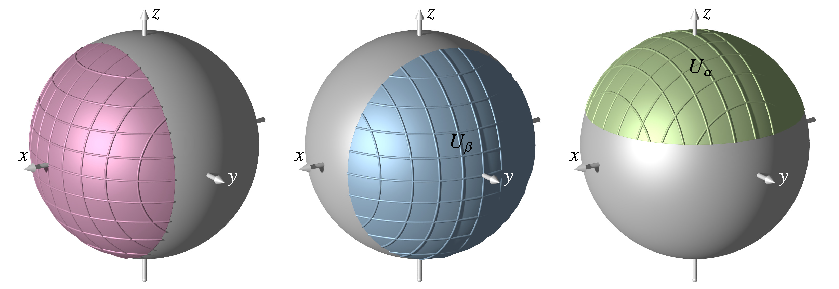
\includegraphics{chapters/030-gruppen/images/kugelkarten.pdf}
%\caption{Drei verschiedene Karten auf einer Kugeloberfläche jeweils in
%einer Umgebung der Schnittpunkte der Kugeloberfläche mit einer
%Achse.
%\label{buch:gruppen:gruppe:fig:kugelkarten}}
%\end{figure}
%Die Menge $S^2 = \{(x,y,z)\mid x^2+y^2+z^2=1\}$ ist eine Kugeloberfläche.
%In der Umgebung $U_\alpha = \{(x,y,z)\in S^2\mid x^2+y^2<0.9\wedge z>0\}$
%des Nordpoles ist die Abbildung
%\[
%\varphi_\alpha
%\colon
%U_\alpha
%:
%(x,y,z)\mapsto (x,y)
%\]
%eine gute Karte, sie deckt aber alle anderen Pole überhaupt nicht ab.
%In der Umgebung $U_\beta = \{(x,y,z)\in S^2\mid x^2+z^2<0.9\wedge y>0\}$
%des Punktes $(0,1,0)$ ist die Abbildung
%\[
%\varphi_\beta
%\colon
%U_\beta
%:
%(x,y,z)\mapsto (x,z)
%\]
%dagegen eine gute Karte.
%So kann für jeden Pol eine Karte gefunden werden, die in 
%Abbildung~\ref{buch:gruppen:gruppe:def:karte} dargestellt sind.
%\end{beispiel}
%
%Das Beispiel zeigt, dass die vollständige Beschreibung einer Menge
%eine Vielzahl von Karten benötigen kann.
%Aus den Koordinatenfunktionen werden dann andere Eigenschaften der
%Menge abgeleietet.
%Dies kann jedoch nur funktionieren, wenn im Überschneidungsbereich
%zweier Koordinatensysteme, die gleichen Eigenschaften abgeleitet
%werden können.
%Im nächsten Abschnitt wird genau dieses Problem für die
%Charakterisierung der Differenzierbarkeit von Funktionen auf der
%Menge adressiert.
%
%%
%% Ableitungen
%%
%\subsubsection{Ableitungen}
%\begin{figure}
%\centering
%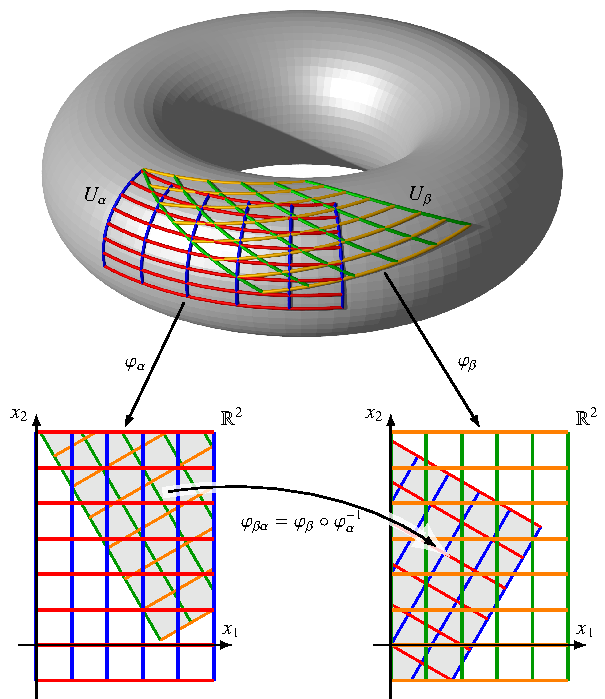
\includegraphics{chapters/030-gruppen/images/karten.pdf}
%\caption{Kartenwechsel für zwei Karten auf einem Torus
%\label{buch:gruppen:gruppe:fig:kartenwechsel}}
%\end{figure}
%Die Karten sollen der Menge $M$ ein Koordinatensystem geben, mit dem
%man Ableitungen von Funktionen definieren kann.
%Dazu ist notwendig, dass verschiedene Karten auf die gleiche
%Ableitung führen.
%Seien $x_i$ und $y_i$ Koordinaten für eine offene Teilmenge von $M$,
%und $f$ eine Funktionen auf $M$.
%In dieser Menge können die Koordinaten $x_i$ als Funktionen der 
%Koordinaten $y_k$ in der Form $x_i(y_1,\dots,y_k)$ schreiben.
%Ebenso kann man $f$ durch die Koordinaten $x_i$ ausdrücken, dies
%schreiben wir als $f(x_1,\dots,x_n)$, oder durch die Koordinaten $y_i$,
%dies schreiben wir als $f(y_1,\dots,y_n)$.
%Die Ableitung der Funktion $f$ nach den Koordinaten $y_i$ muss nach
%der Kettenregel
%\begin{equation}
%\frac{\partial f}{\partial y_i}
%=
%\sum_{k=1}^n
%\frac{\partial f}{\partial x_k} \frac{\partial x_k}{\partial y_i}
%\label{buch:gruppen:gruppe:eqn:kettenregel}
%\end{equation}
%auch durch die Ableitungen von $f$ nach den Koordinaten $y_i$
%ausgedrückt werden können.
%Die Formel~\ref{buch:gruppen:gruppe:eqn:kettenregel} ist aber nur sinnvoll,
%wenn die Ableitungen $\partial x_k/\partial y_i$ alle existieren.
%Die Kartenwelchselabbildung $y\mapsto x$ muss also differenzierbar sein.
%Die Koordinatenumrechnung zwischen zwei Karten müssen also differenzierbare
%Abbildungen sein.
%
%Seien also
%$\varphi_\alpha\colon U_\alpha \to \mathbb{R}^n$
%und
%$\varphi_\beta\colon U_\beta \to \mathbb{R}^n$
%zwei Karten, deren Definitionsbereiche $U_\alpha$ und $U_\beta$ sich
%schneiden.
%Sie statten also beide die Menge $U_{\alpha\beta}=U_\alpha\cap U_\beta$
%mit einem Koordinatensystem aus.
%Die Koordinatenwechselabbildung
%\[
%\varphi_{\beta\alpha}
%=
%\varphi_\beta
%\circ
%\varphi_\alpha^{-1}
%\colon
%\varphi_\alpha(U_\alpha\cap U_\beta)
%\to
%\varphi_\beta(U_\alpha\cap U_\beta)
%\]
%ist eine Abbildung zwischen offenen Teilmengen von $\mathbb{R}^n$.
%Man sagt, der Kartenwechsel ist differenzierbar, wenn $\varphi_{\beta\alpha}$
%differenzierbar ist.
%Der Kartenwechsel in der umgekehrten Richtung ist $\varphi_{\alpha\beta}$.
%
%\begin{definition}
%\label{buch:gruppen:gruppe:def:atlas}
%Ein {\em differenzierbarer Atlas} von $M$ ist eine Menge von Karten derart,
%dass alle Kartenwechselabbildungen differenzierbar sind.
%\end{definition}
%
%\begin{definition}
%\label{buch:gruppen:gruppe:def:diffman}
%Eine {\em differenzierbare Mannigfaltigkeit} ist eine Menge $M$ mit einem
%differenzierbaren Atlas derart, dass jeder Punkt von $M$ im
%Definitionsgebiet mindestens einer Karte liegt.
%\end{definition}
%
%Eine differenzierbare Mannigfaltigkeit ist also eine Menge, die in
%einer Umgebung jedes Punktes mit mindestens einem Koordinatensystem
%ausgestattet werden kann auf eine Art, dass die Umrechnung zwischen
%verschiedenen Koordinatensystemen immer differenzierbar ist.
%
%\begin{beispiel}
%Die reelle Achse $\mathbb{R}$ ist eine differenzierbare Mannigfaltigkeit,
%sie lässt sich mit einer einzigen Karte parametrisieren.
%\end{beispiel}
%
%\begin{beispiel}
%Die Kreislinie $S^1$ in der komplexen Ebene ist eine differenzierbare
%Mannigfaltigkeit, Karten können wie folgt konstruiert werden.
%Die Abbildung $\mathbb{R}\to S^1: x\mapsto e^{ix}$ bildet die ganze
%reelle Achse auf die Kreislinie ab.
%Die Abbildung ist allerdings nicht umkehrbar, weil $x$-Werte, die sich
%um Vielfache von $2\pi$ unterscheiden, auf den gleichen Punkt in $S^1$
%abgebildet werden.
%Zu jedem Punkt $x\in\mathbb{R}$ gibt es aber ein Intervall
%$U_x=(x-1,x+1)$, welches bijektiv auf eine Teilmenge von $S^1$
%abgebildet wird.
%Die Exponentialabbildung von $U_x\to S^1$ wie auch die Umkehrabbildung
%von der Bildmenge zurück in $U_x$ sind stetig.
%Die Koordinaten, die verschiedene solche Karten einem Punkt der Kreislinie
%zuordnen können, unterscheiden sich immer um Vielfache von $2\pi$.
%Die Koordinatenwechsel-Abbildung zwischen zwei Karten $U_x$ und $U_y$
%sind also Abbildungen der Form $x\mapsto x+2\pi k$ mit $k\in\mathbb{Z}$,
%also sicher differenzierbar.
%Damit ist ein differenzierbarer Atlas für $S^1$ konstruiert, $S^1$
%ist eine differenzierbare Mannigfaltigkeit.
%\end{beispiel}
%
%\begin{beispiel}
%\begin{figure}
%\centering
%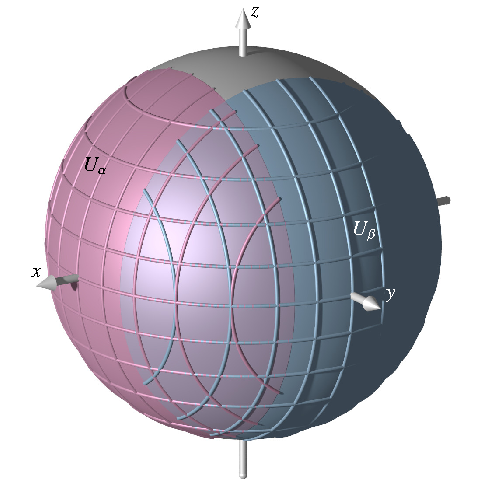
\includegraphics{chapters/030-gruppen/images/kugelschnitt.pdf}
%\caption{Zwei Karten der Kugeloberfläche und deren Schnittbereich.
%Differenzierbarkeit von Funktionen auf der Kugeloberfläche kann mit
%Hilfe der Karten nur dann definiert werden, wenn die Kartenwechselabbildung
%$\varphi_\alpha\circ\varphi_\beta^{-1}$ und
%$\varphi_\beta\circ\varphi_\alpha^{-1}$ differenzierbare Abbildungen
%zwischen offenen Mengen in $\mathbb{R}^n$ sind.
%\label{buch:gruppen:gruppe:fig:kugelkartenwechsel}}
%\end{figure}
%Die Ableitung von Funktionen auf einer Kugeloberfläche muss auf 
%die Beschreibung der Funktion in einer Karte mit Hilfe der dortigen
%Koordinaten zurückführen.
%Dazu ist notwendig, dass die Kartenwelchselabbildungen differenzierbar
%sind.
%Für die in Beispiel~\ref{buch:gruppen:gruppe:bsp:kugel} gezeigten
%Karten auf der Kugeloberfläche ist dies leicht nachzurechnen.
%Das in Abbildung~\ref{buch:gruppen:gruppe:fig:kugelkartenwechsel}
%hat die Kartenwechselfunktion
%\[
%\varphi_\beta
%\circ
%\varphi_\alpha^{-1}
%\colon
%\varphi_\alpha(U_\alpha\cap U_\beta)
%\to
%\varphi_\beta(U_\alpha\cap U_\beta)
%:
%(x,z) \mapsto (x,\!\sqrt{1-x^2-z^2}),
%\]
%die offensichtlich differenzierbar ist, solange $x^2+z^2<1$ ist.
%\end{beispiel}
%
%%
%% Differenzierbare Abbildungen
%%
%\subsubsection{Differenzierbare Abbildungen}
%Ein differenzierbarer Atlas erlaubt jetzt auch Abbildungen zwischen
%verschiedenen Mannigfaltigkeiten zu definieren.
%Sind $M$ und $N$ differenzierbare Mannigfaltigkeiten der Dimension $m$
%bzw.~$n$ und $f\colon M\to N$ eine Abbildung.
%Ist $x\in M$ ein Punkt in $M$, dann gibt es eine Karte
%$\varphi_\alpha\colon U_\alpha\to\mathbb{R}^m$ mit $x\in U_\alpha$
%und eine Karten $\psi_\gamma\colon V_\gamma\to\mathbb{R}^n$ mit
%$f(x)\in V_\gamma$.
%In einer Umgebung von $\varphi_\alpha(x)$ kann die Abbildung $f$
%in den Koordinaten als
%\[
%f_{\gamma,\alpha}
%=
%\psi_\gamma\circ f \circ \varphi_\alpha^{-1}
%\]
%geschrieben werden.
%Als Abbildung einer offenen Menge in $\mathbb{R}^m$ in eine offene
%Menge in $\mathbb{R}^n$ ist wohldefiniert, was es heisst, dass die
%Abbildung differenzierbar ist.
%
%Wählt man andere Karten $\varphi_\beta\colon U_\beta\to\mathbb{R}^n$
%und $\psi_\delta\colon V_\delta\to\mathbb{R}^n$, die ebenfalls
%das Urbild $x\in U_\beta$ und das Bild $f(x)\in V_\delta$ enthalten,
%dann lässt sich die Funktion auch durch die neuen Koordinaten
%\[
%f_{\delta,\beta}
%=
%\psi_\delta\colon \circ f \circ\varphi_\beta^{-1}
%\]
%ausdrücken.
%Natürlich muss auch $f_{\delta,\beta}$ differenuzierbar sein.
%Diese beiden Arten, die Ableitung zu definieren, sind miteinander
%konsistent, weil für die Zusammensetzung
%\[
%f_{\gamma,\alpha}
%=
%\psi_\gamma\circ\psi_\delta^{-1}
%\circ
%f_{\delta,\beta}
%\circ
%\varphi_\beta\circ\varphi_\alpha^{-1}
%=
%\psi_{\gamma\delta}
%\circ
%f_{\delta,\beta}
%\circ
%\varphi_{\beta\alpha}
%\]
%die Kettenregel gilt und die Kartenwechselabbildungen $\varphi_{\beta\alpha}$
%und $\psi_{\gamma\delta}$ differenzierbar sind.
%
%%
%% Lie-Gruppen
%%
%\subsubsection{Lie-Gruppen}
%Die Gruppen $S^1$ war als differenzierbare Mannigfaltigkeit erkannt
%worden.
%Damit die Struktur der Gruppe und die differenzierbare Struktur sinnvoll
%miteinander verwendet werden können ist notwendig, dass die
%Verknüpfungsabbildung $(x,y)\mapsto xy$ und die Umkehrabbildung
%$x\mapsto x^{-1}$ nicht nur stetig, sondern sogar differenzierbar sind.
%
%\begin{definition}
%\label{buch:gruppen:gruppe:def:liegruppe}
%Eine Lie-Gruppe ist eine Gruppe, die gleichzeitig eine differenzierbare
%Mannigfaltigkeit ist derart, dass die Gruppenoperation
%$G\times G\to G:(x,y)\mapsto xy$
%und die Invertierung $G\to G: x\mapsto x^{-1}$ differenzierbare Abbildungen
%sind.
%\end{definition}
%
%In den für die Gruppe $S^1$ konstruierten Karten ist die Verknüpfung die
%Addition von Koordinaten und die Invertierung ist der Vorzeichenwechsel.
%Beide sind differenzierbar, daher ist $S^1$ eine Lie-Gruppe.
%
%%
%% Koordinatensysteme auf Matrizengruppen
%%
%\subsubsection{Koordinatensysteme auf Matrizengruppen}
%Die allgemeine lineare Gruppe $\operatorname{GL}_n(\mathbb{R})$
%ist eine offene Teilmenge von $\mathbb{R}^{n\times n}$ ist.
%Die Matrixelemente $a_{ik}$ sind daher auf natürliche Weise ein
%Koordinatensystem auf der Gruppe $\operatorname{GL}_n(\mathbb{R})$.
%Die Gruppenoperationen lassen sich als Summen von Produkten von
%Matrixelementen schreiben.
%Mit den Matrixelementen als Koordinaten folgt unmittelbar, dass
%die Gruppenoperationen differenzierbare Abbildungen sind.
%
%Alle anderen Matrizengruppen sind Teilmengen von
%$\operatorname{GL}_n(\mathbb{R})$ niedrigerer Dimension.
%Zum Beispiel besteht die Gruppe $\operatorname{SL}_n(\mathbb{R})$
%aus den Matrizen mit Determinante $1$, der $(n^2-1)$-dimensionalen
%Teilmenge von $\operatorname{GL}_n(\mathbb{R})$ bestehend aus
%den Nullstellen der Gleichung $\det(A)-1=0$.
%Die Gruppe $\operatorname{SO}(n)$ besteht aus den Matrizen, die
%zusätzlich $A^tA=I$ erfüllen.
%Da $A^tA$ eine symmetrische Matrix ist, sind dies
%$n(n+1)/2$ unabhängige Bedinungen.
%Da daraus auch $\det A=\pm$ folgt, ist die $n(n-1)/2$ Dimension der Gruppe
%$\operatorname{SO}(n)$, denn
%\[
%n^2 - \frac{n(n+1)}2
%=
%\frac{2n^2-n^2-n}{2}
%=
%\frac{n^2-n}2
%=
%\frac{n(n-1)}2.
%\]
%Da diese Einschränkungen ausserdem differenzierbar sind und in der
%Einheitsmatrix keine Singularitäten haben, kann man davon ausgehen,
%dass diese Teilmengen Untermannigfaltigkeiten sind.
%
%Kann man auf kanonische Art Karten für die Matrizengruppen
%konstruieren?
%Die Matrixform der Rodrigues-Formel (\cite[p.~438]{buch:linalg})
%beschreibt Drehungen des dreidimensionalen Raumes um die Achse mit
%Richtung des Einheitsvektors $\vec{u}$ und um den Drehwinkel $\alpha$a
%durch die Matrix
%\[
%D_{\vec{u},\alpha}
%=
%\begin{pmatrix}
% 1-(1-c)(1-u_1^2) & -su_3+(1-c)u_1u_2 &  su_2+(1-c)u_1u_3 \\
% su_3+(1-c)u_1u_2 &  1-(1-c)(1-u_2^2) & -su_1+(1-c)u_2u_3 \\
%-su_2+(1-c)u_1u_3 &  su_1+(1-c)u_2u_3 &  1-(1-c)(1-u_3^2) 
%\end{pmatrix}
%\]
%beschrieben werden kann.
%Der Vektor $\vec{u}$ ist ein Einheitsvektor und daher $\vec{u}\in S^2$
%ein Punkt auf einer Kugel.
%Wählt man auf der Kugel eine Karte, kann man daraus zusammen mit den
%Drehwinkeln eine Karte für die Drehmatrizen konstruieren.
%Dies zeigt, dass $\operatorname{SO}(3)$ eine differenzierbare
%Mannigfaltigkeit ist.
%
%Die Konstruktion des vorangeangenen Absatzes ist nicht direkt
%auf andere Matrizengruppen verallgemeinerbar.
%Man kann aber zeigen, dass in einer Umgebung der Einheitsmatrix
%sich die Matrizen einer Matrizengruppe mit Hilfe der Exponentialreihe
%schreiben lassen (siehe auch \cite[Abschnitt~9.4.4]{buch:linalg}).
%Zum Beispiel sind die Matrizen $A\in \operatorname{SL}_n(\mathbb{R})$
%in einer Umgebung von $I$ von der Form
%\(
%e^U
%\),
%wobei
%die  Matrix $U$ Spur $\operatorname{tr}{U}=0$ haben muss.
%Die Menge der Matrizen mit Spur $0$ ist eine $(n^2-1)$-dimensionale
%Teilmenge von $M_{n}(\mathbb{R})$.
%Die Umkehrabbildung der Exponentialabbildung kann daher als Karte
%in einer Umgebung von $I$ dienen.
%
%Ganz allgemein ist die Exponentialabbildung immer eine lokal
%invertierbare Abbildung von der Lie-Algebra einer Matrizengruppe
%in die Lie-Gruppe.
%Da die Lie-Algebra ein $\mathbb{R}$-Vektorraum ist, kann eine
%lokale Umkehrabbildung um die Einheitsmatrix $I$ als Karte mit
%Werten in der Lie-Algebra dienen.
%Für die Gruppe $\operatorname{SO}(3)$ zum Beispiel besteht die
%Lie-Algebra aus antisymmetrischen Matrizen, also Matrizen
%der Form
%\[
%U
%=
%\begin{pmatrix}
%  0  & -u_3 &  u_2 \\
% u_3 &   0  & -u_1 \\
%-u_2 &  u_1 &   0
%\end{pmatrix}.
%\]
%Die Exponentialabbildung ordnet der Matrix $U$ die Matrix $e^U$
%zu, die nach der Exponentialform der Rodrigues-Formel 
%(\cite[p.~483]{buch:linalg}) die Drehmatrix der Drehung um die
%Achse mit Richtung $\vec{u}^0$ und mit Drehwinkel $\alpha=|\vec{u}|$
%ist, wobei $\vec{u}$ der Vektor mit den Komponenten $u_1$, $u_2$ und
%$u_3$ ist.
%Das Tripel $(u_1,u_2,u_3)$ bildet also ein gutes Koordinatensystem
%für eine Umgebung der Einheitsmatrix in der Gruppe $\operatorname{SO}(3)$.
%
%Die aus der Lie-Algebra konstruierten Karten zeigen noch mehr.
%Da die Exponentialabbildung beliebig oft differenzierbar ist und die
%Matrixmultiplikation durch Polynome höchstens zweiten Grades in
%den Matrixelementen ausgedrückt werden kann, sind die Koordinatenwechsel
%immer beliebig oft differenzierbar.
%Die Matrizengruppen sind also sogar beliebig oft differenzierbare
%Mannigfaltiketen. 
%Es ist daher zulässig, sich für die Zwecke der nachfolgenden Diskussionen
%immer auf beliebig oft differenzierbare Funktionen einzuschränken.
%Andere, weniger oft differenzierbare Funktionen können durch
%solche Funktionen beliebig genau approximiert werden.

%%
%% Funktionen auf einer Gruppe
%%
%\subsection{Funktionen auf einer Gruppe
%\label{buch:gruppen:subsection:funktionen}}
%In diesem Abschnitt ist $G$ eine Gruppe, die wir multiplikativ
%schreiben.
%Die harmonische Analysis handelt von der Analyse von Funktionen.
%Im Falle einer Lie-Gruppe kann man zusätzlich sinnvoll von Ableitungen
%der Funktionen sprechen.
%Wir definieren daher
%
%\begin{definition}
%\label{buch:gruppen:gruppe:def:funktionenaufgruppe}
%Die Menge der stetigen reell- und komplexwertigen Funktionen wird mit
%$C_{\mathbb{R}}(G)$ bzw.~$C_{\mathbb{C}}(G)$ bezeichnet.
%Ist $G$ eine Lie-Gruppe, dann ist
%$C_{\mathbb{R}}^\infty(G)$ die Menge der unendlich oft differenzierbaren
%reellwertigen Funktionen auf $G$,
%$C_{\mathbb{C}}^\infty(G)$ ist die Menge der unendlich oft differenzierbaren
%komplexwertigen Funktionen.
%\end{definition}
%
%Die Gruppenstruktur ermöglich, lineare Operatoren auf $C_{\mathbb{R}}(G)$
%und $C_{\mathbb{C}}(G)$ zu definieren.
%
%\begin{definition}
%\label{buch:gruppen:gruppe:def:translation}
%Für $s\in G$ ist $T_s$ die Abbildung
%\[
%T_s
%\colon
%C_{\mathbb{R}}(G) \to C_{\mathbb{R}}(G)
%:
%f \mapsto T_sf
%\quad
%\text{mit}
%\quad
%(T_sf)(x) = f(s^{-1}x).
%\]
%Sie heisst die {\em Translation} um $s\in G$.
%\end{definition}
%
%Die Translation ist natürlich linear, denn
%\begin{align*}
%(T_s(f+g))(x)
%&=
%(f+g)(s^{-1}x)
%\\
%&=
%f(s^{-1}x) + g(s^{-1}x)
%=
%(T_sf)(x) + (T_sg)(x)
%&&\Rightarrow&
%T_s(f+g)&=T_sf+T_sg
%\\
%(T_s(\lambda f))(x)
%&=
%\lambda f(s^{-1}x)
%=
%\lambda (T_sf)(x)
%&&\Rightarrow&
%T_s\lambda f
%&=
%\lambda T_sf
%\end{align*}
%
%%
%% Eigenvektoren von T_s
%%
%\subsubsection{Eigenfunktionen des Translationsoperators}
%Tatsächlich wurden in früheren Kapiteln Funktionen verwendet, die
%bezüglich der Translation besondere Eigenschaften hatten.
%Zum Beispiel sind die Funktionen $f(x)=e_k(x)=e^{ikx}$ auf $G=\mathbb{R}$
%Eigenfunktionen des Translationsoperators, denn
%\[
%(T_se_k)(x)
%=
%e^{ik(x-s)}
%=
%e^{iks}e^{ikx}
%=
%e^{-iks} e_k(x).
%\]
%Insbesondere ist $e_k$ eine Eigenfunktion von $T_s$ mit Eigenwert
%$\lambda=e^{-iks}$, also $T_se_k = \lambda e_k$.
%
%%
%% Gruppenstruktur der Translationen
%%
%\subsubsection{Gruppenstruktur der Translationen}
%Wir berechnen die Zusammensetzung zweier Translationen ist $T_s$ und $T_t$.
%Um $T_sT_t$ zu berechnen, muss zunächst die Funktion $T_tf$ bestimmt werden.
%Es ist $(T_tf)(x) = f(t^{-1}x)$.
%Die Translation $T_sg$ einer beliebigen Funktion auf dem Element $y\in G$
%ist $(T_sg)(y)=g(s^{-1}y)$.
%Setzt man $g=T_tf$ ein, ergibt sich
%\[
%(T_sT_tf)(x)
%=
%(T_tf)(s^{-1}x)
%=
%f(t^{-1}s^{-1}x)
%=
%f((st)^{-1}x)
%=
%(T_{st}f)(x),
%\]
%also $T_sT_t=T_{st}$.
%
%%
%% Rechtsoperation der Gruppe auf 
%%
%\subsubsection{Rechtsoperation von $G$ auf $C(G)$}
%Die Operation $T_s$ ist genauer die Links-Translation, die Gruppenoperation
%wirkt auf das Argument von links.
%Für eine abelsche Gruppe spielt die Reihenfolge der Operanden keine
%Rolle, für eine nichtabelsche Gruppe ergibt sich jedoch ein Unterschied.
%
%\begin{definition}
%Der Operator $R_s\colon C(G)\to C(G)$ der Rechts-Translation ist definiert
%durch
%\[
%R_s
%\colon
%C_{\mathbb{R}}(G)\to C_{\mathbb{R}}(G)
%:
%f \mapsto R_sf
%\quad\text{mit}\quad
%(R_sf)(x) = f(xs).
%\]
%\end{definition}
%
%Die Zusammensetzung von $R_s$ und $R_t$ kann ganz ähnlich wie für
%$T_s$ und $T_t$ berechnet werden.
%Zunächst ist $R_sg(y) = g(ys)$.
%Wendet man dies auf $g=R_tf$ mit $g(x)=(R_tf)(x)=f(xt)$ an, bekommt man
%\[
%(R_sR_tf)(x)
%=
%(R_sg)(x)
%=
%g(xs)
%=
%(R_tf)(xs)
%=
%f(xst)
%=
%(R_{st}f)(x)
%\]
%oder kurz $R_sR_t=R_{st}$.
%
%
%
%
